%\documentclass[a4paper,10pt]{article} % 11pt

\documentclass[letterpaper,10pt]{article} % 10pt
%Use article for short documents
%\usepackage[T1]{fontenc}
\usepackage{parskip}
\usepackage{latexsym,amsmath,amssymb}
%\usepackage{natbib}
\usepackage{graphicx}
%\usepackage{times}
\usepackage{zi4}
\usepackage[letterpaper,left=4cm,right=4cm,top=3cm,bottom=3cm]{geometry}
%\usepackage[a4paper,left=4cm,right=4cm,top=3cm,bottom=3cm]{geometry}



\usepackage[nottoc,numbib]{tocbibind} % References in contents?


\pagestyle{myheadings} % page numbers on top right

\thispagestyle{empty}

\title{Polygenic Markov Chain}
\author{Jesse Murray}
\date{}

\begin{document}
\maketitle


\pagenumbering{arabic}



\section*{Abstract}
%
A Markov chain model of polygenic inheritance is proposed.
%
Population members reproduce in discrete time, i.e., generations, and have phenotypic scores in continuous space.
%
The initial condition is a standard normal distribution of scores.
%
The one-step transition (parent to offspring score) is a normal linear model, which is determined by the regression and residual coefficients.
%
From this formulation, many important properties are derived. 
%
Given a present score, conditional distributions for the scores of all descendants and ancestors are found. 
%
These conditional distributions are normal, furthermore, their expectation and variance have exponential functions over time, i.e., the generation-gap.
%
As expected, the conditional distributions converge to the marginal population distribution as the generation-gap widens.
%
The regression and residual coefficients determine the rates of convergence such that a robust measure of mobility -- equivalently, information loss -- is introduced as the ratio of the residual to the regression coefficient.
%
Stable population variance is defined as the case where the marginal population variance remains constant over generations.
%
This occurs when the sum of the two squared coefficients equals one, and results in a reversible stationary distribution, meaning the model of inheritance behaves identically going forwards and backwards in time.
%
The Markov chain is shown to have probability kernels that can make important predictions over any number of generations in the form of probability attributable and probability destined, which are equivalent in percentile transition matrices. 
%
From two large datasets, the proposed model is shown to accurately describe the inheritance of human stature -- with complete confirmation under stable population variance.



\newpage

% CONTENTS
\tableofcontents
\clearpage


%\section{Introduction}
%A simple Markov chain model is proposed that seeks to describe the movement of polygenic scores between familial generations. Some potentially useful %properties are shown to result from this model. %The model is compared with the data on the statures of 898 adult children and their parents, as collected by Francis Galton. 



%% MODEL FORMULATION %%
\section{Model formulation}

\subsection{Analogy to polygenic inheritance}
Polygenic inheritance occurs when a trait is determined by many genes (up to hundreds or thousands). In general, the observed phenotypic scores of polygenic traits are normally distributed, which results from the central limit theorem \cite{rieger}. That is, the genotype is the additive sum of many small gene-effects, which are independent and can have an arbitrary probability distribution \cite{lange_book}. 

A Markov chain is proposed that seeks to provide a basic model for the multi-generational dynamics of inheritance for a univariate polygenic trait. One example of such a trait is human stature, which is thought to be a non-sex-linked, nondominant, polygenic trait \cite{luo}. The observed normal distribution of human stature is unsurprising as, at the time of this writing, there have been 697 variants identified at genome-wide significance that together explain only one-fifth of heritability for adult height \cite{preece, wood}. 

Until now, simple normal linear models have been used to predict offspring height from parent height. However, these linear models have not been generalized in the form of a Markov chain. 

\subsection{Markov chain model of inheritance}

% COMPLETE DESCRIPTION

The proposed Markov chain exists in discrete time $ i \in \{0, 1, 2,...\}$, where $i$ is the familial generation (parent, offspring, etc.); and continuous space $X_i \in \mathbb{R}$, where $X_i$ is the phenotypic score of the analogized univariate polygenic trait. The terms \emph{score} and \emph{state} are used interchangeably in reference to the phenotypic score. 

\begin{description}
\item [Convention] Let $Z$ refer to a generic standard normal $Z \sim \mathcal{N}(0, 1)$. The mentions of $Z$ throughout the text are used for explanatory purposes and they can be assumed to be unassociated with one another unless specified otherwise.
\item [Convention] We will use the tilde symbol, e.g. $\tilde{\mu}_{i+n}$, to denote the conditional parameters, such as conditional expectation and variance, that describe an upward or downward (conditional) transition distribution.
\end{description}

The proposed Markov chain can be entirely derived from: (1.) the initial condition and (2.) the one-step downward transition. 

\begin{enumerate}
\item The initial score is drawn from a standard normal distribution representing the scores of the initial generation: $X_0 \sim \mathcal{N}(0, 1)$. A normally distributed univariate polygenic trait can be standardized to meet this condition. 

\item The conditional one-step downward transition, i.e., the score of an offspring, given the score of its parent, is also drawn from a normal distribution: $X_{i+1}|X_i \sim \mathcal{N}(\tilde{\mu}_{i+1}, \tilde{\sigma}_{i+1}^2)$.
$$X_{i+1}|X_i = \tilde{\mu}_{i+1} + \tilde{\sigma}_{i+1} Z$$ 

\begin{enumerate}
\item An offspring's score is proportional to the score of its parent, which is scaled by $r$ -- the \emph{regression coefficient}. In order for there to be regression towards the population mean, we require $0 < r < 1$. 
$$\tilde{\mu}_{i+1} = \mathrm{E}(X_{i+1}|X_i) = rX_i$$

\item While the expected offspring's score can be calculated from the score of its parent, there is a normally distributed residual about the expected offspring score that has a standard deviation (SD) equal to the marginal SD of the parent generation scaled by $r_s$ -- the \emph{residual coefficient}. For the residual SD to be positive and a degenerate normal distribution avoided, we require $r_s > 0$.
$$\tilde{\sigma}_{i+1} = \sqrt{\mathrm{Var}(X_{i+1}|X_i)} = r_s \sigma_i$$
\end{enumerate}
\end{enumerate}

\subsubsection{Brief and complete description of the chain}
As we have shown, the Markov chain can be constructed from the equations for the initial condition and the one-step downward transition:
$$X_0 \sim \mathcal{N}(0, 1)$$
$$X_{i+1}|X_i = rX_i+ r_s\sigma_iZ$$
The latter equation contains the important coefficients $r$ and $r_s$, which have been named the regression coefficient and the residual coefficient, respectively. 

\subsubsection*{Note about standardization to real data}
The distribution of the initial generation was set to $X_0 \sim \mathcal{N}(0, 1)$, and it was briefly mentioned that the phenotypic score of any univariate polygenic trait, e.g. stature, which is measured in centimeters, could be standardized to have mean zero and variance one. Due to this initial standardization, the scores of all generations are given in z-scores relative to the initial generation. Therefore, in order to obtain a score in terms its measured units, e.g., centimeters, one need only shift and scale the score by the mean and SD, respectively, of the initial generation. 

When handling real data, it may be the case that one has the measured mean and SD of some other generation besides the initial generation. In that case, it is worth noting that the mean of all generations is zero under this model. Furthermore, the SD of any generation can be easily calculated with $r$ and $r_s$ from the SD of any other generation.



% NORMAL LINEAR 
\subsection{Linear regression form}

The one-step downward transition of the Markov chain can be written:
$$X_{i+1} = rX_i + \epsilon$$
$$\epsilon \sim \mathcal{N}(0, r_s^2 \sigma_i^2)$$

This has the same form as a normal linear model of one variable, in which the explanatory variable is normally distributed. We begin with the paired column vectors $\bold{x}, \bold{y}$, both containing $n$ data points. The vectors could contain the statures of mothers and daughters after standardization to the mothers' mean and SD. 
$$\bold{y} = r \, \bold{x} + \bold{\epsilon}$$
$$\bold{\epsilon} \sim \mathcal{N}(\bold{0}, r_s^2 I_n)$$
$$\bold{x} \sim \mathcal{N}(\bold{0}, I_n)$$

Where $\bold{0}$ is a vector of length $n$ containing zeros, and $I_n$ is the $n \times n$ identity matrix, and the vector $\epsilon$ represents the errors, or differences in statures $\bold{y}$ from the predicted statures $r\bold{x}$. 

\subsubsection*{Without standardization}
The column vectors $\bold{x}, \bold{y}$ were both standardized to the mean and SD of the measured parent scores. It is easy to show how the linear regression equation can be written in terms of the un-standardized scores $\bold{x}_u, \bold{y}_u$ of the parents and offspring, which might be the measurements in their original units, e.g. centimeters. 
$$\bold{y}_u =  r \, \bold{x}_u + \sigma_x\bold{\epsilon} +  \bold{\mu}_x(1-r)$$
Where $\bold{\mu}_x$ is a repeated column vector containing the mean of the parent scores and $\sigma_x$ is the standard deviation of the parent scores, both given in their measured units. Importantly, the regression coefficient is still the slope of the regression line, even without standardization. 


\subsubsection*{Estimating $r$ and $r_s$ from one-step transition data}
It can be shown that the maximum likelihood estimate (MLE) of $r$ is obtained by minimizing the sum of the squared errors. 
%
$$\hat{r} = (\bold{x}^T \bold{x})^{-1} \bold{x}^T \bold{y}$$
%
The MLE of $r_s^2$ is obtained from the minimum value of the sum of squared errors. That is, $\hat{r}_s^2$ is equal to the variance of $\epsilon$, under the MLE of $r$. Taking the square root to obtain the MLE of $\hat{r}_s$, we get:
%
$$\hat{r}_s = \sqrt{\mathrm{Var}({\epsilon} | \hat{r})}$$%

These equations gives us a way to obtain the MLEs of $r$ and $r_s$ from one-step transition data. 



% ASSUMPTIONS AND LIMITATIONS
\subsection{Assumptions and limitations}

\subsubsection*{Assumptions}
\begin{enumerate}
\item Normality of the polygenic trait. This assumption is generally supported by the literature consensus on the effect of the central limit theorem for additive polygenic traits. The normality assumption has been widely been confirmed within the literature on human stature \cite{luo}.
\item Normal linear relationship between parent and offspring statures. That is, the linear regression form of the one-step downward transition has normally distributed residuals. This has been verified for human stature \cite{luo}.
\item Equal probability and degree of successful reproduction for all members of the population -- regardless of score. In other words, no members of the population have more offspring than other members, and no natural selection occurs. 
\item Phenotypes are determined in the absence of net environmental effects, which would directionally shift phenotypic scores between generations. It is shown however, that an environmental effect that acts uniformly on the population as a whole can easily be included in the model. 
\end{enumerate}

\subsubsection*{Limitations}
\begin{enumerate}
\item No average movement of the population mean occurs between generations due to the equal probability of successful reproduction and no net environmental effects. Therefore, all generations have marginal population mean zero.
\item Marginal populations implicitly exist in discrete time and are non-overlapping, each having mean $0$ and SD $\sigma_i^2$.
\item Population size is not modeled. 
\item Over many generations ($n$-step transitions for when $n$ is large), the model appears to be more appropriate under the condition of stable population variance. Otherwise, the population variance eventually expands to $\infty$ or shrinks to $0$, depending on whether $r^2 + r_s^2$ is greater than one or less than one, respectively. On the other hand, it will be discussed how proposed calculations of probability attributable and probability destined can remain valid and undistorted even when there is unstable population variance.
\end{enumerate}


\subsubsection*{Adjustment for uniform environmental effects}
It is worth remarking on the historical observation of human heights increasing between generations, which has been attributed to improvements in the environment for growth, in terms of nutrition and health \cite{bogin}. Previous studies have suggested that overall improvements in access to food, dietary diversification, sanitation, water, living standards, and decreasing exposure to disease are responsible for the secular increases in height occurring in the 19th and 20th centuries across many developed countries \cite{perkins}. 

As was discussed in the limitations section, the model proposed here does not describe average movement of the population mean between generations as a result of net-environmental effects that would uniformly shift the conditional mean of each offspring. However, we can fortunately include these effects in the model without causing any problems. Here, we denote $c$ by the increase in height between generations:
$$X_{i+1} = r(X_i - \mu_i) + \epsilon + c$$

Then, the change to our model is quite straightforward, and can be given entirely by the change to the marginal population mean, which until now has always been zero.
$$\mu_{i+n} = \mu_i + nc$$
Likewise, we have:
$$\mu_{i-n} = \mu_i - nc$$
We need only add the $\mu_{i \pm n}$ adjustment to all of the conditional expectations described throughout -- (all of the variances will remain unaffected). 

Alternatively, if $c$ varies over time (given by the generation number), such that $c(i)$ may be greater than or less than $c(j)$, we get the following form for the adjustment:
$$\mu_{i+n} = \mu_i + \sum_{t = i+1}^{i+n} c(t)$$
$$\mu_{i-n} = \mu_i - \sum_{t = i-1}^{i-n} c(t)$$

Note that the convergences to the marginal distributions are not affected as the adjustment constant is added to both the marginal and conditional expectation, and thus cancels out when the two are compared. 

The observation of increasing height between generations does not affect the integrity of the un-adjusted form of the model, as we have discussed how increases in height have resulted from improved environmental factors, rather than genetic inheritance per se. It is then fair to say that the model seeks to describe polygenic inheritance -- in the absence of net environmental effects, such as improving nutrition. However, such effects can easily be included within the model if necessary, as long as they act uniformly on all offspring. This is shown to be the case in both the large population-based and historical Pearson datasets. 





%% PROPERTIES %%
\section{Properties}
\subsection{Marginal population distribution}
The unconditional (marginal) distribution of a population member's score can be shown by induction and the theorem of the sum of independent normal random variables (rvs) to be given by $X_n \sim \mathcal{N}(0, \sigma_n^2)$, which can also be written:
$$X_n = \sigma_nZ$$

This occurs because the residuals of the one-step downward transition are normally distributed about the conditional expectation. If the residuals were not normally distributed, the population would depart from the normal distribution in the next generation.

\begin{description}
\item [Definition] Let $\sigma_i^2$ -- the \emph{population variance} -- refer to the marginal variance of $X_i$, i.e., without the knowledge of any past or future score $X_{j}$, with $j \neq i$. The population variance is shown to be related to the population variance of a previous generation. Likewise, the \emph{population variance} can be shown to always remain zero under the model. 
\end{description}

Then, for $Z_\alpha$, $Z_\beta$ iid standard normals, the marginal random state $X_{i+1}$ can be written in terms of the population variance of the previous state.
$$X_{i+1} = r\sigma_iZ_\alpha + r_s\sigma_iZ_\beta$$

\subsubsection*{Population variance}
From the equation for the marginal random state $X_{i+1}$, it can be shown that $\sigma_{i+1}^2$ has the following one-step relationship with the previous population variance:
$$\sigma_{i+1}^2 = (r^2+r_s^2)  \sigma_i^2$$
By induction, the population variance can be computed from a previous population variance for an arbitrary step-length:
$$\sigma_{i+n}^2 = (r^2+r_s^2)^n  \sigma_{i}^2$$




% COVARIANCE AND CORRELATION
\subsection{Covariance and correlation}
The regression coefficient relates to the covariance and correlation between the scores of an ancestor and its descendant. Recall that when $n = 1$, we are then describing parent and offspring. 
$$\mathrm{Cov}(X_{i+n}, X_i) = r^n \sigma_i^2$$
$$\mathrm{Corr}(X_{i+n}, X_i) = r^n \frac{\sigma_i}{\sigma_{i+n}}$$






% CONDITIONAL DESCENDANT DISTRIBUTION
\subsection{Conditional descendant distribution}

In describing the chain, we gave the conditional one-step downward transition, which was the rv of an offspring's score as a function of its parent's score. However, we would like to have a general expression for the probability distribution of  a descendant's score given its ancestor's score, for any number of generations $n$ separating the two. 

The conditional distribution $X_{i+n}|X_i$ can be shown to be normally distributed with the following expressions for $\mathrm{E}(X_{i+n}|X_i)$ and $\mathrm{Var}(X_{i+n}|X_i)$:

$$X_{i+n}|X_i \sim \mathcal{N}( \tilde{\mu}_{i+n}, \tilde{\sigma}_{i+n}^2)$$

$$\tilde{\mu}_{i+n} = r^nX_i$$

$$\tilde{\sigma}_{i+n}^2 = [(r^2+r_s^2)^n-r^{2n}] \sigma_i^2$$

The equation for conditional variance results from continually re-applying the one-step downward transition, which leads to the following equation for $X_{i+n}|X_i$:
$$X_{i+n}|X_i = r^nX_i + r_s\sigma_i \sum_{j=1}^{n}r^{n-j}(r^2+r_s^2)^{\frac{j-1}{2}}Z_j$$

It might appear that in order to obtain $\tilde{\sigma}_{i+n}^2$, we would need to make the unpleasant summation of the squared coefficients that multiply each $Z_j$. However, the earlier equation for population variance can be deployed, in which $r^nX_i$ is treated as a random variable instead of a constant. Then, the population variance is equal to the sum of marginal variance of $r^nX_i$ and $\tilde{\sigma}_{i+n}^2$.
%
$$\sigma_{i+n}^2 =  (r^2+r_s^2)^n  \sigma_{i}^2 =  r^{2n}\sigma_i^2 + \tilde{\sigma}_{i+n}^2$$
%
After rearranging and taking the square root, we obtain the equation for $\tilde{\sigma}_{i+n}$.

Our result is consistent with the following fact, which can be shown by induction to hold for all real numbers $a$,  $b$:
$$(a+b)^n = a^n + b \sum_{j=1}^{n}a^{n-j}(a+b)^{j-1}$$

In the section on the conditional ancestor distribution, we will show another way the conditional descendant distribution can be obtained.




%% DOWNWARD CONVERGENCE
\subsection{Exponential convergence of the conditional descendant distribution}

\subsubsection*{Convergence to the marginal distribution}
The conditional distribution of a descendant's score, given its ancestor's score $X_{i+n}|X_i \sim \mathcal{N}( \tilde{\mu}_{i+n}, \tilde{\sigma}_{i+n}^2)$ converges to its marginal population distribution of $X_{i+n}$ for large $n$.

Under regression towards the mean, we have $0 < r < 1$, for which we get the following convergence for large $n$:
$$r^n \rightarrow 0$$
This convergence affects the conditional expectation, which converges to the marginal (population) mean:
$$\tilde{\mu}_{i+n} = r^nX_i \rightarrow 0$$
Likewise, the convergence of $r^n$ affects the conditional variance $\mathrm{Var}(X_{i+n}|X_i)$, which can be written:
$$\tilde{\sigma}_{i+n}^2 = \sigma_{i+n}^2 - r^{2n} \sigma_i^2$$
This equation can perhaps more helpfully be written as a ratio:
$$\frac{\tilde{\sigma}_{i+n}^2}{\sigma_{i+n}^2} = 1 - (\frac{r^2}{r^2+r_s^2})^n$$
Recalling that the chain required $r_s > 0$, we see that the conditional variance converges to the population variance for large $n$:
$$\tilde{\sigma}_{i+n}^2 \rightarrow \sigma_{i+n}^2$$

In summary, as $n \rightarrow \infty$:
$$X_{i+n}|X_i \rightarrow X_{i+n}$$

By the polygenic analogy, this result says that after many generations, a population member's descendants will have scores that become asymptotically indistinguishable from the marginal scores of the population. In other words, as more generations separate an ancestor and its descendant, the ancestor's score becomes asymptotically useless for predicting the descendant's score.


\subsubsection*{Role of the coefficients}
The rate at which the conditional descendant distribution converges to the population distribution is determined by the regression and residual coefficients. 

From the expressions for the downward convergence in expectation as well as in variance, we see that the more regression towards the mean there is (\emph{smaller $r$}), the faster the downward convergence to the marginal distribution. Likewise, the less regression towards the mean there is (\emph{larger $r$}), the slower the downward convergence to the marginal distribution. 

From the expression for the downward convergence in variance, we that the less residual variance there is (\emph{smaller $r_s$}), the slower the convergence to the marginal distribution. That is, as long as $|r| < 1$, otherwise the conditional expectation will not converge to $0$. Likewise, the larger the residual variance (\emph{larger $r_s$}), the faster the convergence to the marginal distribution. 


\subsubsection*{Degenerate lower bound for the residual coefficient}
We can show that $r \geq r^2 + r_s^2$ is essentially degenerate, resulting in a lower bound on $r_s$:
$$r_s > \sqrt{r(1-r)}$$

The possible values for $r$ and $r_s$ due to their initial requirements and this newly given lower bound on $r_s$ are shown in Figure \ref{fig:possible_r_rs}. 

\begin{figure}[h]
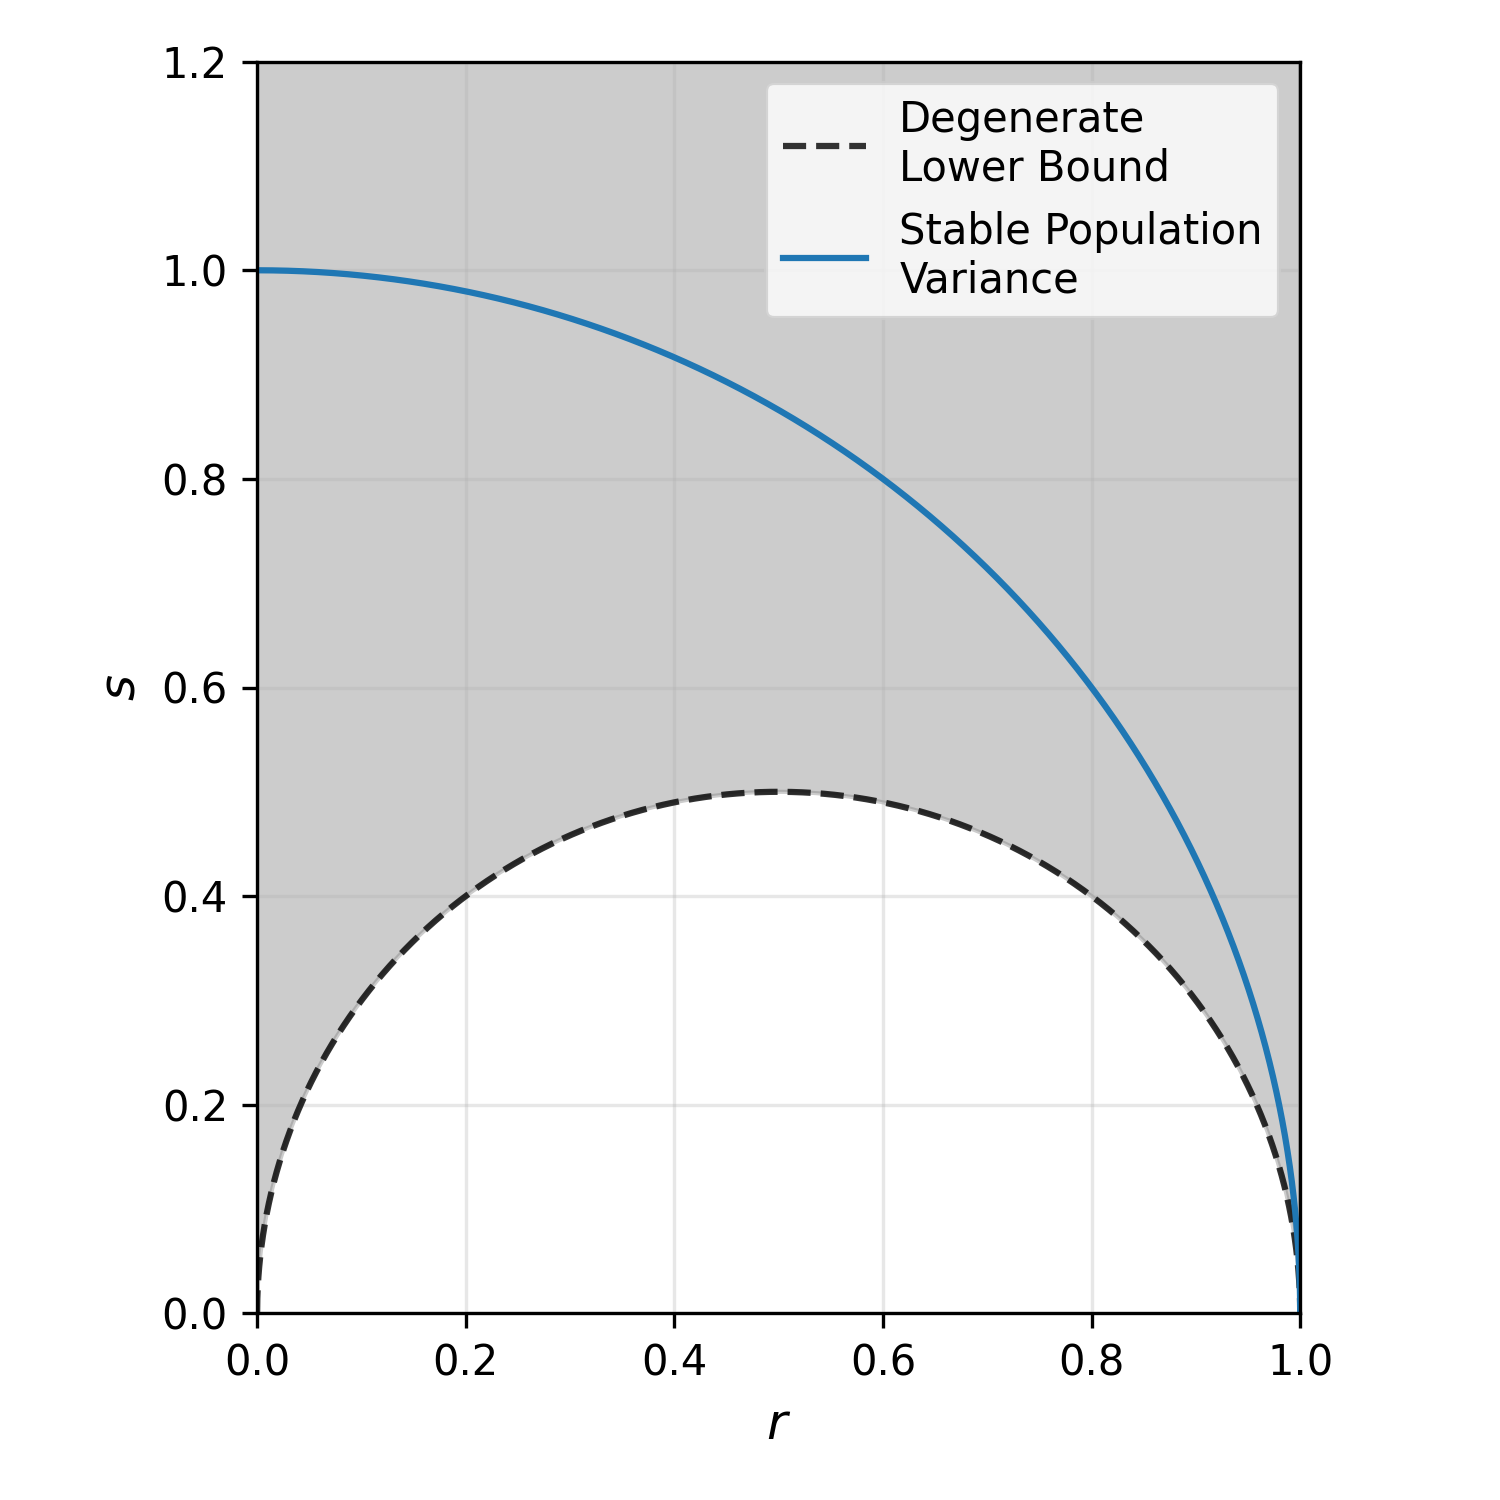
\includegraphics[width=3in]{figures/possible_r_rs.png}
\centering
\caption{Possible values for the regression and residual coefficients are given by the shaded area, which extends upwards for $r_s \rightarrow \infty$. The degenerate lower bound has $r_s > \sqrt{r(1-r)}$ and stable population variance (the stationary distribution) has $r_s = \sqrt{1-r^2}$.}
\label{fig:possible_r_rs}
\end{figure}

We can show why breaching this lower bound is degenerate by breaking up $r \geq r^2 + r_s^2$ into two cases.

In the first case: $r = r^2 + r_s^2$, then we have no regression to the mean relative to the population variances. In other words, all ancestors have the same expected z-score.
$$\frac{\tilde{\mu}_{i+n}}{\sigma_{i+n}^2} = \frac{X_i}{\sigma_i^2}$$


In the second case: $r > r^2 + r_s^2$, then we have $r^2 + r_s^2 < 1$ and $\sigma_{i+n}^2 \rightarrow 0$ for large $n$, as we have previously shown. While this is otherwise alright, here it leads to the variance of the marginal population shrinking to zero faster than the conditional expectation does, which causes the descendant's expected z-score to diverge.
$$\frac{\tilde{\sigma}_{i+n}^2}{\sigma_{i+n}^2} = (\frac{r}{r^2+r_s^2})^n \frac{X_i}{\sigma_i^2} \rightarrow \infty$$
As $X_i$ was arbitrary, all descendants' expected z-scores would diverge regardless of their ancestors' scores, which can be considered degenerate. 


\subsubsection*{Exponential functions for conditional expectation and variance}

The role of the coefficients can also be seen in the equations for the rate of change in the parameters of the conditional descendant distribution.

The rate of change in the conditional expectation is negative and increasing with $n$ (positive second partial derivative). Therefore, the conditional expectation asymptotically approaches zero, and the smaller $r$ is, the larger the negative rate. The natural logarithm is denoted by '$\log$'.
$$\frac{\partial }{\partial n}[\tilde{\mu}_{i+n}] = -\log(\frac{1}{r}) \, \tilde{\mu}_{i+n}$$


Likewise, the rate of change in the ratio of the conditional variance to the marginal variance is positive and decreasing with $n$ (negative second partial derivative). Therefore, the ratio asymptotically approaches one. The smaller $r$ is, or the larger $r_s$ is, the larger the positive rate of convergence.
$$\frac{\partial }{\partial n}[\frac{\tilde{\sigma}_{i+n}^2}{\sigma_{i+n}^2}] = \log(1+\frac{r_s^2}{r^2}) \, [1 - \frac{\tilde{\sigma}_{i+n}^2}{\sigma_{i+n}^2}]$$

We then get the following exponential functions:
$$\tilde{\mu}_{i+n} = X_i \, \exp[-\log(\frac{1}{r}) \, n]$$
$$\tilde{\sigma}_{i+n}^2 = \sigma_{i+n}^2 \, (1 - \exp[-\log(1+\frac{r_s^2}{r^2}) \, n])$$

Earlier, we derived the conditional distribution of the score of a descendant, given the score of its ancestor $X_{i+n}|X_i \sim \mathcal{N}( \tilde{\mu}_{i+n}, \tilde{\sigma}_{i+n}^2)$. Now we have just shown that the parameters of this distribution are both exponential functions of the generation gap $n$, and that both converge on the marginal parameters. In other words, the conditional expectation of a descendant's score exponentially approaches the population mean, and the conditional variance of a descendant's score also exponentially approaches the population variance. 




% POPULATION VARIANCE
\subsection{Population variance dynamics}

\subsubsection*{Unstable population variance}
We have shown that:
$$\sigma_{i+n}^2 = (r^2+r_s^2)^n  \sigma_{i}^2$$

Taking the limit $n \rightarrow \infty$: 
\begin{itemize}
\item For $r^2+r_s^2 < 1$ we have $\sigma_{i+n}^2 \rightarrow 0$.
\item For  $r^2+r_s^2 > 1$, we have $\sigma_{i+n}^2 \rightarrow \infty$. 
\end{itemize}

These degenerate limits could be prevented if $r$ or $r_s$ were inversely proportional to some power of the population variance $\sigma_i^2$. However, this negative feedback is not explored here. Instead, we discuss the simplest resolution to population variance instability, which is that $r^2+r_s^2 = 1$. Then, every generation has the same population variance.

\subsubsection*{Stable population variance}
We are particularly interested in the case where the population variance remains constant between generations. This would model a population in which the phenotypes of the polygenic trait do not become increasingly or decreasingly spread out between successive generations. 
$$\sigma_{i+1}^2 = \sigma_i^2$$
This occurs if and only if:
$$r^2+r_s^2 = 1$$
%
By induction, the population variance of any arbitrary generation $i$ is equal to the initial variance. 
$$\sigma_i^2 = 1$$



% STATIONARY DISTRIBUTION
\subsection{Stationary distribution}

\subsubsection*{Stable population variance implies stationary distribution}
It can be shown that the chain is at a stationary distribution when there is stable population variance:
$$X_i \sim \mathcal{N}(0, 1)$$
$$X_{i+1} = r Z_\alpha + r_s Z_\beta$$
$$X_{i+1} \sim \mathcal{N}(0, r^2+r_s^2)$$
$$X_{i+1} \sim \mathcal{N}(0, 1)$$

\subsubsection*{Stationary distribution is reversible}
It will be shown in the section on the conditional ancestor distribution that the chain behaves identically going forwards and backwards in time when there is stable population variance.

\subsubsection*{Convergence to the stationary distribution}

From the downward convergence to the marginal distribution and the fact that the stationary distribution is reversible, it follows that the conditional normal distribution converges to the distribution of stationary population. 
As $n \rightarrow \infty$:
$$X_{i+n}|X_i \rightarrow \mathcal{N}(0, 1)$$
$$X_{i-n}|X_i \rightarrow \mathcal{N}(0, 1)$$



%% CONDITIONAL ANCESTOR DISTRIBUTION %%
\subsection{Conditional ancestor distribution}

Up until this point, we have only discussed the conditional random variable of a descendant's score given its ancestor's score. We would however like to be able to describe the upward relationship: the probability distribution of an ancestor's score given its descendant's score, for any number of generations $n$ separating the two. 

\begin{description}
\item [Convention] In order to remain consistent with our earlier notation, it will be easiest to think of the generation number of the ancestor as also $b = i - n$. That is, the ancestor existed at time $b$, which is $n$ generations \emph{before} the current time $i$. 
\end{description}

One way to obtain the distribution of $X_{i-n}|X_i$ is with Bayes' rule. 
$$f(x_{i-n}|x_i) \propto f(x_{b+n}|x_b) f(x_b)$$
This is similar, though not identical, to finding the posterior distribution for $\mu$ of a normal distribution when the prior distribution for $\mu$ is normal. Then, a normal prior times the normal likelihood gives a normal posterior. However, because $X_{b+n}|X_b \sim \mathcal{N}(r^n X_b, \tilde{\sigma}_{b+n}^2)$, such that the $r^n$ term obfuscates the conjugate prior, this approach requires unpleasant algebra for completing the square in the exponent. 

An alternative approach is to recognize that $X_{i-n}$ and $X_i$ form a bivariate normal distribution. Then, the conditional distribution of $X_{i-n}$ given $X_i$ must be normally distributed with the following parameters:
$$\mathrm{E}(X_{i-n}|X_i) = \mathrm{E}(X_{i-n}) + \frac{\mathrm{Cov}(X_{i-n}, X_i)}{\mathrm{Var}(X_i)}[X_i - \mathrm{E}(X_i)]$$
$$\mathrm{Var}(X_{i-n}|X_i) = \mathrm{Var}(X_{i-n}) - \frac{[\mathrm{Cov}(X_{i-n}, X_i)]^2}{\mathrm{Var}(X_i)}$$

Using our earlier results and simplifying, we get that the conditional distribution $X_{i-n}|X_i$ is normally distributed with the following expressions for $\mathrm{E}(X_{i-n}|X_i)$ and $\mathrm{Var}(X_{i-n}|X_i)$:

$$X_{i-n}|X_i \sim \mathcal{N}( \tilde{\mu}_{i-n}, \tilde{\sigma}_{i-n}^2)$$

$$\tilde{\mu}_{i-n} = (\frac{r}{r^2+r_s^2})^n X_i$$

$$\tilde{\sigma}_{i-n}^2 = [1 - (\frac{r^2}{r^2+r_s^2})^n] \sigma_{i-n}^2$$

The bivariate normal approach can also be used to confirm our earlier expressions for $\tilde{\mu}_{i+n}$ and $\tilde{\sigma}_{i+n}^2$, which were previously obtained by continually re-applying the one-step downward transition of the Markov chain.

\subsubsection*{One-step upward transition}
The one-step upward transition describes the conditional distribution of a parent's score given its offspring's score. We can show that $X_{i-1}|X_i \sim \mathcal{N}( \tilde{\mu}_{i-1}, \tilde{\sigma}_{i-1}^2)$ with the following parameters:
$$\tilde{\mu}_{i-1} = \frac{r}{r^2+r_s^2} X_i$$
$$\tilde{\sigma}_{i-1}^2 = \frac{r_s^2}{r^2+r_s^2} \sigma_i^2$$

This has a very similar form to the one-step downward transition, only the coefficients have changed slightly.
$$X_{i-1} = \frac{r}{r^2+r_s^2} X_i + \frac{r_s}{\sqrt{r^2+r_s^2}} \sigma_{i} Z$$


\subsubsection*{Stationary distribution is reversible}

Because we have $r^2+r_s^2 = 1$ under stable population variance, ie., the stationary distribution, the chain behaves the same way going forwards and backwards in time:
$$X_{i-1} = r X_i + r_s \sigma_{i} Z$$
It is straightforward to show that $X_{i-n}|X_i \sim \mathcal{N}( \tilde{\mu}_{i-n}, \tilde{\sigma}_{i-n}^2)$ has the same form as $X_{i+n}|X_i \sim \mathcal{N}( \tilde{\mu}_{i+n}, \tilde{\sigma}_{i+n}^2)$ under the stationary distribution:
$$\tilde{\mu}_{i-n} = \tilde{\mu}_{i+n} = r^nX_i$$
$$\tilde{\sigma}_{i-n}^2 = \tilde{\sigma}_{i+n}^2 = 1-r^{2n}$$





% UPWARD CONVERGENCE
\subsection{Exponential convergence of the conditional ancestor distribution}

\subsubsection*{Convergence to the marginal distribution}
The conditional distribution of an ancestor's score, given its descendant's score $X_{i-n}|X_i \sim \mathcal{N}( \tilde{\mu}_{i-n}, \tilde{\sigma}_{i-n}^2)$ converges to the marginal population distribution of $X_{i-n}$ for large $n$.

Then, for large $n$, we have the following convergences:
$$(\frac{r}{r^2+r_s^2})^n \rightarrow 0$$
$$(\frac{r^2}{r^2+r_s^2})^n \rightarrow 0$$

Therefore, we have convergence both in conditional expectation and variance:
$$\tilde{\mu}_{i-n} \rightarrow 0$$
$$\tilde{\sigma}_{i-n}^2 \rightarrow \sigma_{i-n}^2$$
In summary, as $n \rightarrow \infty$:
$$X_{i-n}|X_i \rightarrow X_{i-n}$$

We have thus confirmed our earlier stated lower bound on $r_s$, as the upward conditional expectation would not converge under the degenerate condition.


\subsubsection*{Role of the coefficients}
The rate at which the conditional ancestor distribution converges to the population distribution is determined by the regression and residual coefficients. 

It is worth noting that the ratio of the downward conditional variance to the marginal variance is the same as the ratio of the upward conditional variance to the marginal variance, shown earlier. Therefore, the effects of $r$ and $r_s$ are the same for both the upward and downward convergence of conditional variance to the marginal variance.

From the expressions of convergence for both expectation and variance, we see that a smaller regression coefficient $r$ leads to faster convergence, and vice versa; and that a smaller residual coefficient $r_s$ leads to slower convergence, and vice versa. Unlike in the downward convergence, upward convergence does not require $|r| < 1$.

\subsubsection*{Exponential functions for conditional expectation and variance}
The role of the coefficients can also be seen in the equations for the rate of change in the parameters of the conditional ancestor distribution.

The rate of change in the conditional expectation is negative and increasing with $n$ (positive second partial derivative). Therefore, the conditional expectation asymptotically approaches $0$. The smaller $r$ is, or the larger $r_s$ is, the larger the negative rate. 
$$\frac{\partial}{\partial n}[\tilde{\mu}_{i-n}] = -\log(\frac{r^2 + r_s^2}{r}) \, \tilde{\mu}_{i-n}$$

The rate of change in the ratio of the conditional variance to the marginal variance has the same form as in the upward convergence. Therefore, the rate of change is positive and decreasing with $n$ (negative second partial derivative), asymptotically approaching one. The smaller $r$ is, or the larger $r_s$ is, the larger the positive rate of convergence.
$$\frac{\partial }{\partial n}[\frac{\tilde{\sigma}_{i-n}^2}{\sigma_{i-n}^2}] = \log(1+\frac{r_s^2}{r^2}) \, [1 - \frac{\tilde{\sigma}_{i-n}^2}{\sigma_{i-n}^2}]$$

We then get the following exponential functions:
$$\tilde{\mu}_{i-n} = X_i \, \exp[-\log(\frac{r^2 + r_s^2}{r}) \, n]$$
$$\tilde{\sigma}_{i-n}^2 = \sigma_{i-n}^2 \, (1 - \exp[-\log(1+\frac{r_s^2}{r^2}) \, n])$$

Earlier, we derived the conditional distribution of the score of an ancestor, given the score of its descendant $X_{i-n}|X_i \sim \mathcal{N}( \tilde{\mu}_{i-n}, \tilde{\sigma}_{i-n}^2)$. Now we have just shown that the parameters of this distribution are both exponential functions of the generation gap $n$, and that both converge on the marginal parameters. In other words, the conditional expectation of an ancestor's score exponentially approaches the population mean, and the conditional variance of an ancestor's score also exponentially approaches the population variance. 









%% MODEL VERIFICATION FOR HUMAN STATURE %%
\section{Application to human stature}

The model formulation is checked against data on the heights of parents and their adult children. Because all of the properties of the Markov chain follow from the initial condition and the one-step downward transition, confirming their accuracy confirms the model's properties over any number of steps.

\subsubsection*{Verifying the model}
We consider the parental generation to be the initial generation. Then, we have two basic requirements to confirm our model:
\begin{enumerate}
\item The parental heights are modeled by the initial condition.
\item The conditional distribution of the offspring heights is modeled by the one-step downward transition, for which we can also refer to its linear regression form.
\end{enumerate}



\subsection{Large population-based study}

The study \emph{Target Height as Predicted by Parental Heights in a Population-Based Study}, published in \emph{Nature -- Pediatric Research} \cite{luo}, analyzed the relationship between the heights of adult children and the heights of their parents for predicting target height. The data they analyzed was from a large sample ($n$ = 2402) of normal Swedish children born in the 1970s. 


\subsubsection*{The initial condition}
Unfortunately, the authors did not report on the normality of the parental heights in the dataset. Nonetheless, the authors cite a paper that reports height to be normally distributed in a population \cite{preece}. Thus, we can assume that the parental heights were normally distributed, confirming the initial condition.


\subsubsection*{The one-step downward transition}

An increase in height between generations was observed, amounting to 0.7 cm for male and 1.0 cm for female subjects. We have shown that as long as the increase is uniform, i.e., not dependent on the parent's score, then we can include the increase in the model by the addition of a constant-term in the linear regression. That is, as long as the mean residual values are zero over all possible parent scores, then the increase is uniform and is accurately described by the adjustment to the model.

The authors tested the validity of a normal linear model for the one-step transition of parent to offspring heights. Their model was identical to the linear regression form of the one-step transition discussed earlier. The authors confirm the veracity of the linear model, and thus the they confirm the formulation one-step downward transition -- completely in the case of stable population variance.

The authors confirm the validity of the normal linear model by the following tests:
\begin{enumerate}
\item The residuals were normally distributed (tested by skewness and kurtosis).
\item The mean residual values were fairly constant over the range of midparental heights, fluctuating around zero, and were only statistically significantly above zero ($p < 0.05$) for very short mid-parental heights (below $-2$ SDs).
\item The mean residual values were constant over the range of difference in parental heights.
\item The residual SDs were constant over the range of midparental height  
\item The residual SDs were constant over the range of difference in parental heights.
\end{enumerate}

In summary, the residuals were normally distributed about the linearly predicted offspring height, and neither midparental height, nor the difference in parental height, affected the residual values. In terms of the model, this result means that both $r$ and $r_s$ are neither dependent on $X_i$, nor on the difference between $X_i$ and the score of the mating partner. 

The authors also conclude that the predictive accuracy was also not affected by assortative mating, as they observed a correlation coefficient between the parents of 0.27, which is an indication of assortative mating.



\subsubsection*{Observed coefficients}
Varied values of $r$ and $r_s$ were found for using mothers' heights to predict sons' heights, fathers' heights to predict sons' heights, mothers' heights to predict daughters' heights, etc. However, these four possibilities averaged around $r$ = 0.49 and $r_s$ = 0.88, which essentially produces stable population variance, giving a ratio of the adult children's SD to the parents' SD, which we will from now on call the SD ratio, of 1.01.
$$\mathrm{SD} \, \mathrm{ratio} = \frac{\sigma_{i+1}}{\sigma_i}$$

\subsubsection*{Model can be completely confirmed for stable population variance}
From one-step transition data, we cannot confirm the part of our model that says $\tilde{\sigma}_{i+1} = r_s \sigma_i$, that is, except for when there is stable population variance. Then, $\sigma_i$ is constant, and we have $\tilde{\sigma}_{i+1} = r_s$, because the initial variance is standardized to one.

In the dataset, the observed ratio of the sons-fathers SD ratio was 0.978, consistent with stable population variance. The observed ratio of the daughters-mothers SD ratio was 1.16, somewhat consistent with stable population variance. 

It is possible that members towards the outer edges of the population distribution of height are less likely to have offspring -- or have fewer offspring -- than those towards the middle, which would have the effect of counteracting otherwise expanding population variance. On the other hand, if this is not observed, then it is reasonable to assume that the stable population variance condition applies to human stature, in which case the resultant stationary distribution and all of its properties apply as well. 



\subsection{Historic dataset}

Karl Pearson organized the collection of data on over 1,100 families in England in the 1890s. The dataset he collected contains the heights of mothers, fathers and their adult children with no more than two adult children per family \cite{pearson}. All of adult children were at least age 18, and all of the parents were at most 65 years of age. Here, we check the validity of the model by verifying the initial condition and the one-step downward transition. We present this in detail for the daughter-mother data ($n$ = 1375). Though not shown here, the model passed all of the exact same statistical tests for the son-father data ($n$ = 1078).


\subsubsection*{The initial condition}

It is obvious from the Q-Q plot in Figure \ref{fig:qq_pearson_x} that the mother's scores are normally distributed. Furthermore, the normality assumption passes statistical tests of skewness and kurtosis, as well as D’Agostino and Pearson's test that combines skew and kurtosis to produce a single test of normality.

\begin{figure}[h]
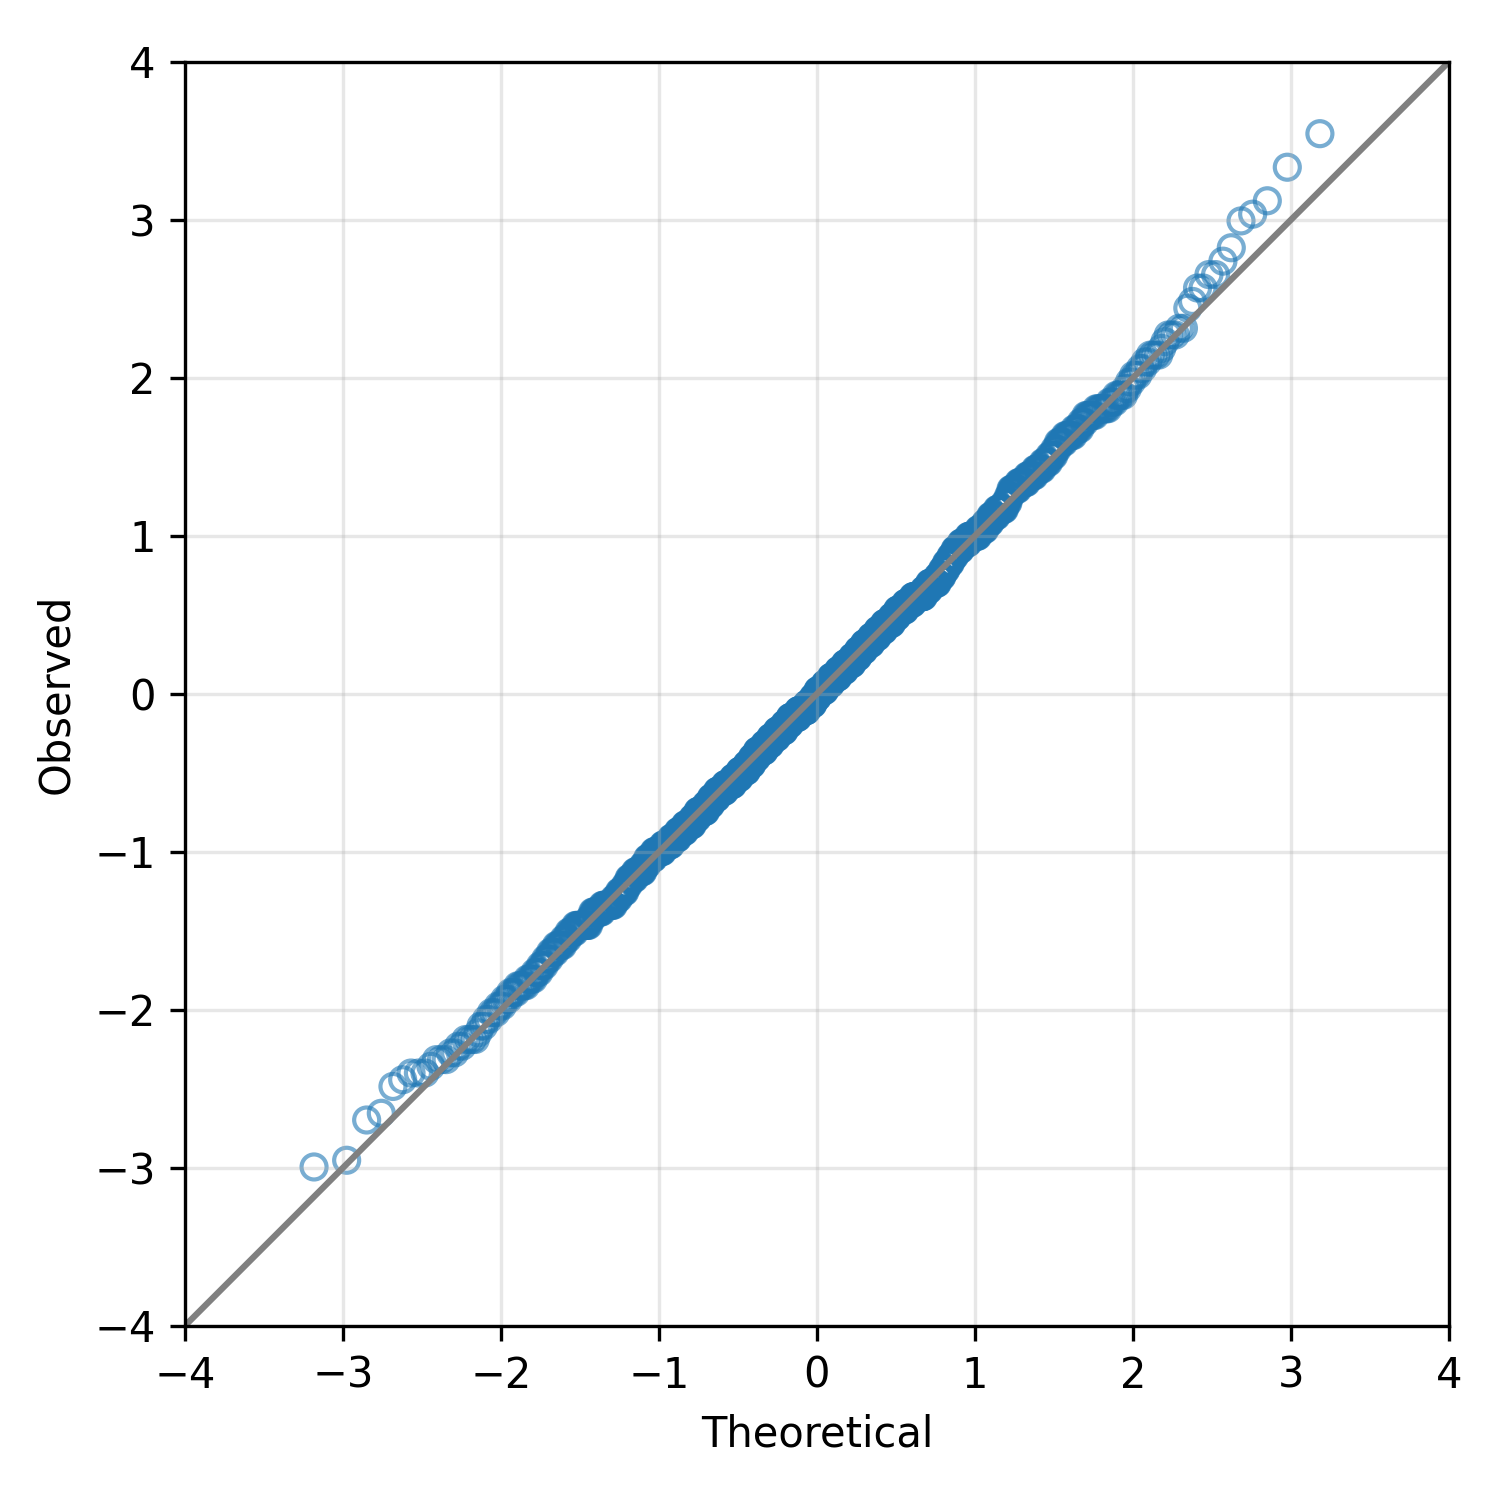
\includegraphics[width=3in]{figures/qq_pearson_x.png}
\centering
\caption{Q-Q plot of the mothers' scores in the Pearson female dataset.}
\label{fig:qq_pearson_x}
\end{figure}


\subsubsection*{The one-step downward transition}

As in the Swedish data, an increase in height between generations was observed, amounting to 3.3 cm, meaning that the adjustment to our model must be made. 

We can see that the residuals were normally distributed from the Q-Q plot in Figure \ref{fig:qq_pearson_epsi}. Furthermore, the normality assumption passes statistical tests of skewness, kurtosis, and D’Agostino and Pearson's test.

Likewise, we can show in Figure \ref{fig:pearson_residuals_by_score} that the residuals have mean zero over all parent scores. This means that the adjustment constant can be applied safely as the shift applies uniformly to all offspring. 


\begin{figure}[p]
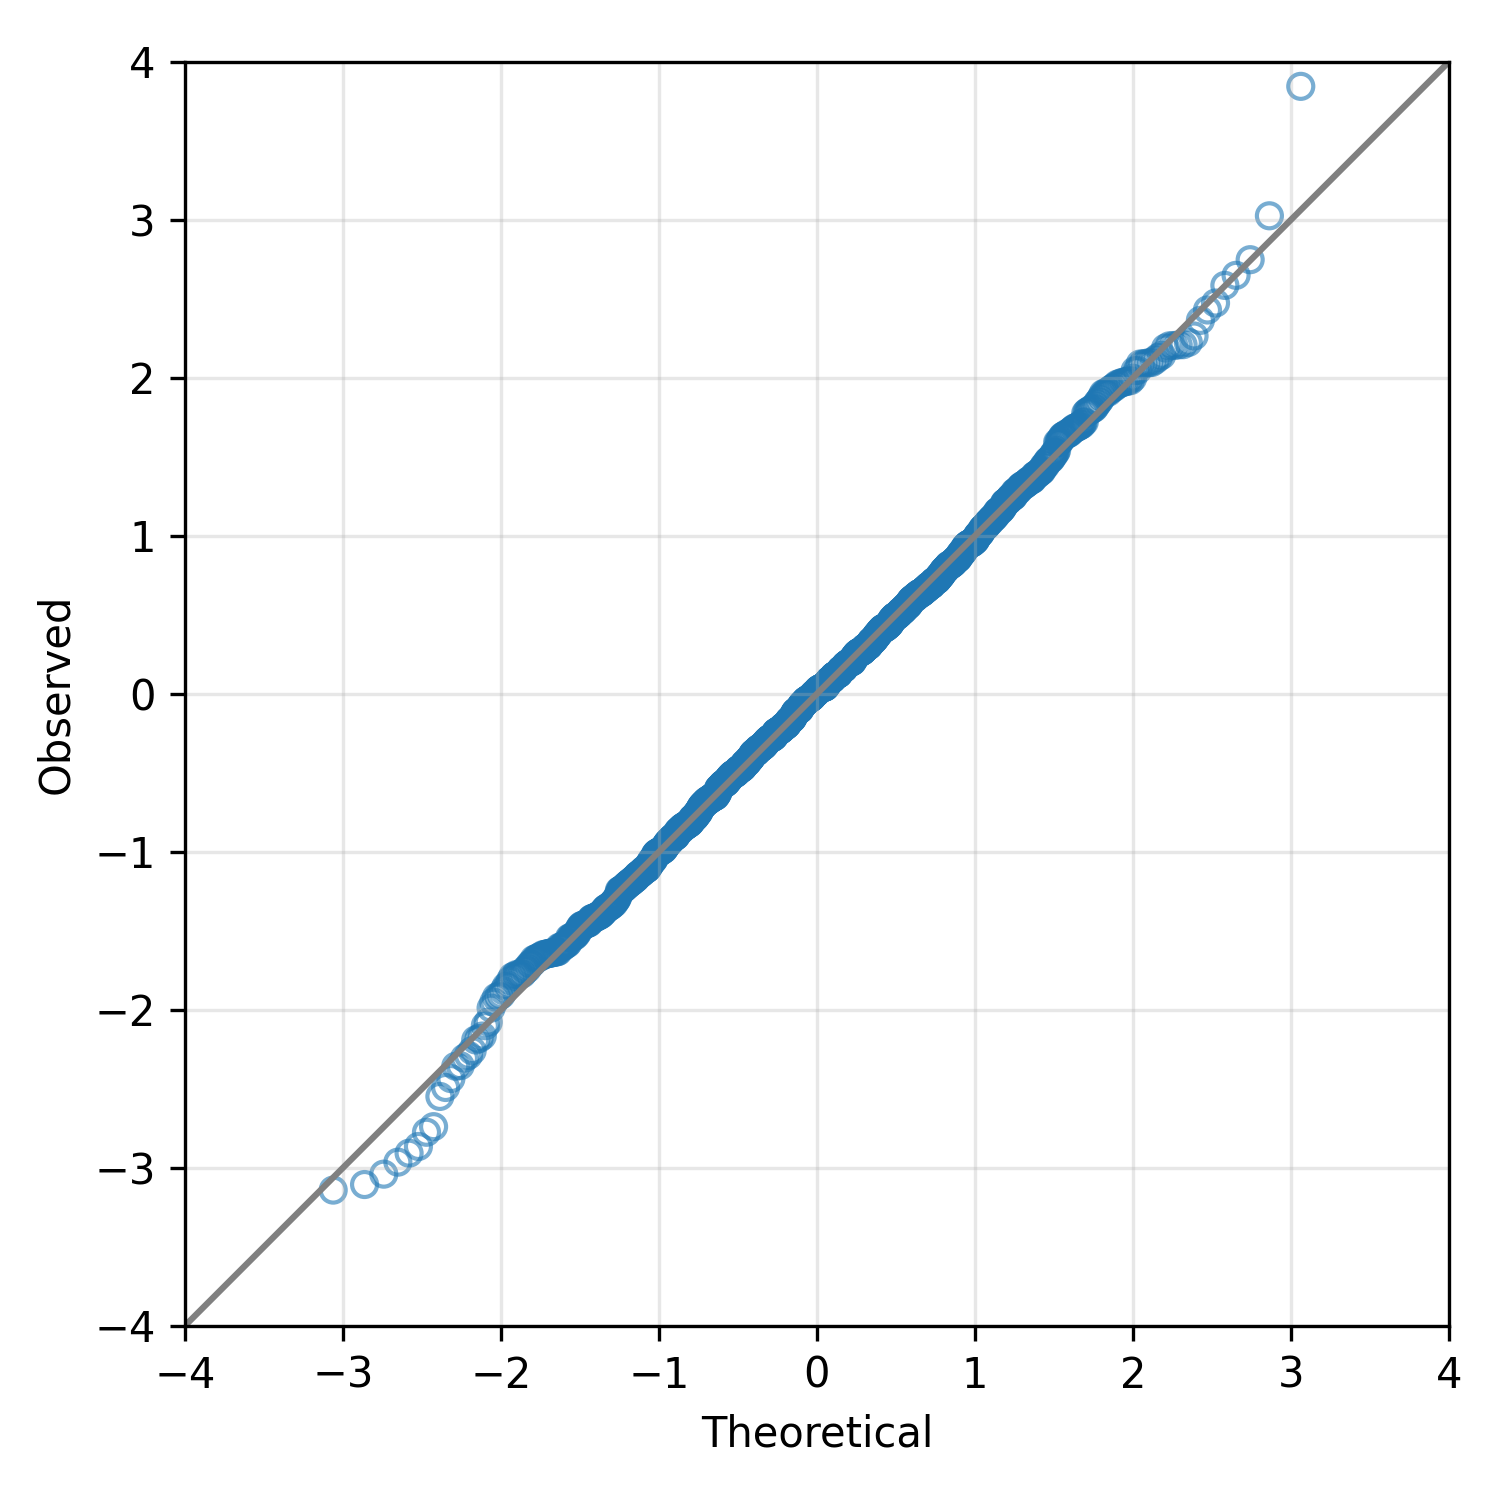
\includegraphics[width=3in]{figures/qq_pearson_epsi.png}
\centering
\caption{Q-Q plot of the daughters' residuals in the Pearson female dataset.}
\label{fig:qq_pearson_epsi}
%\end{figure}

\vspace{2cm}

%\begin{figure}[h]
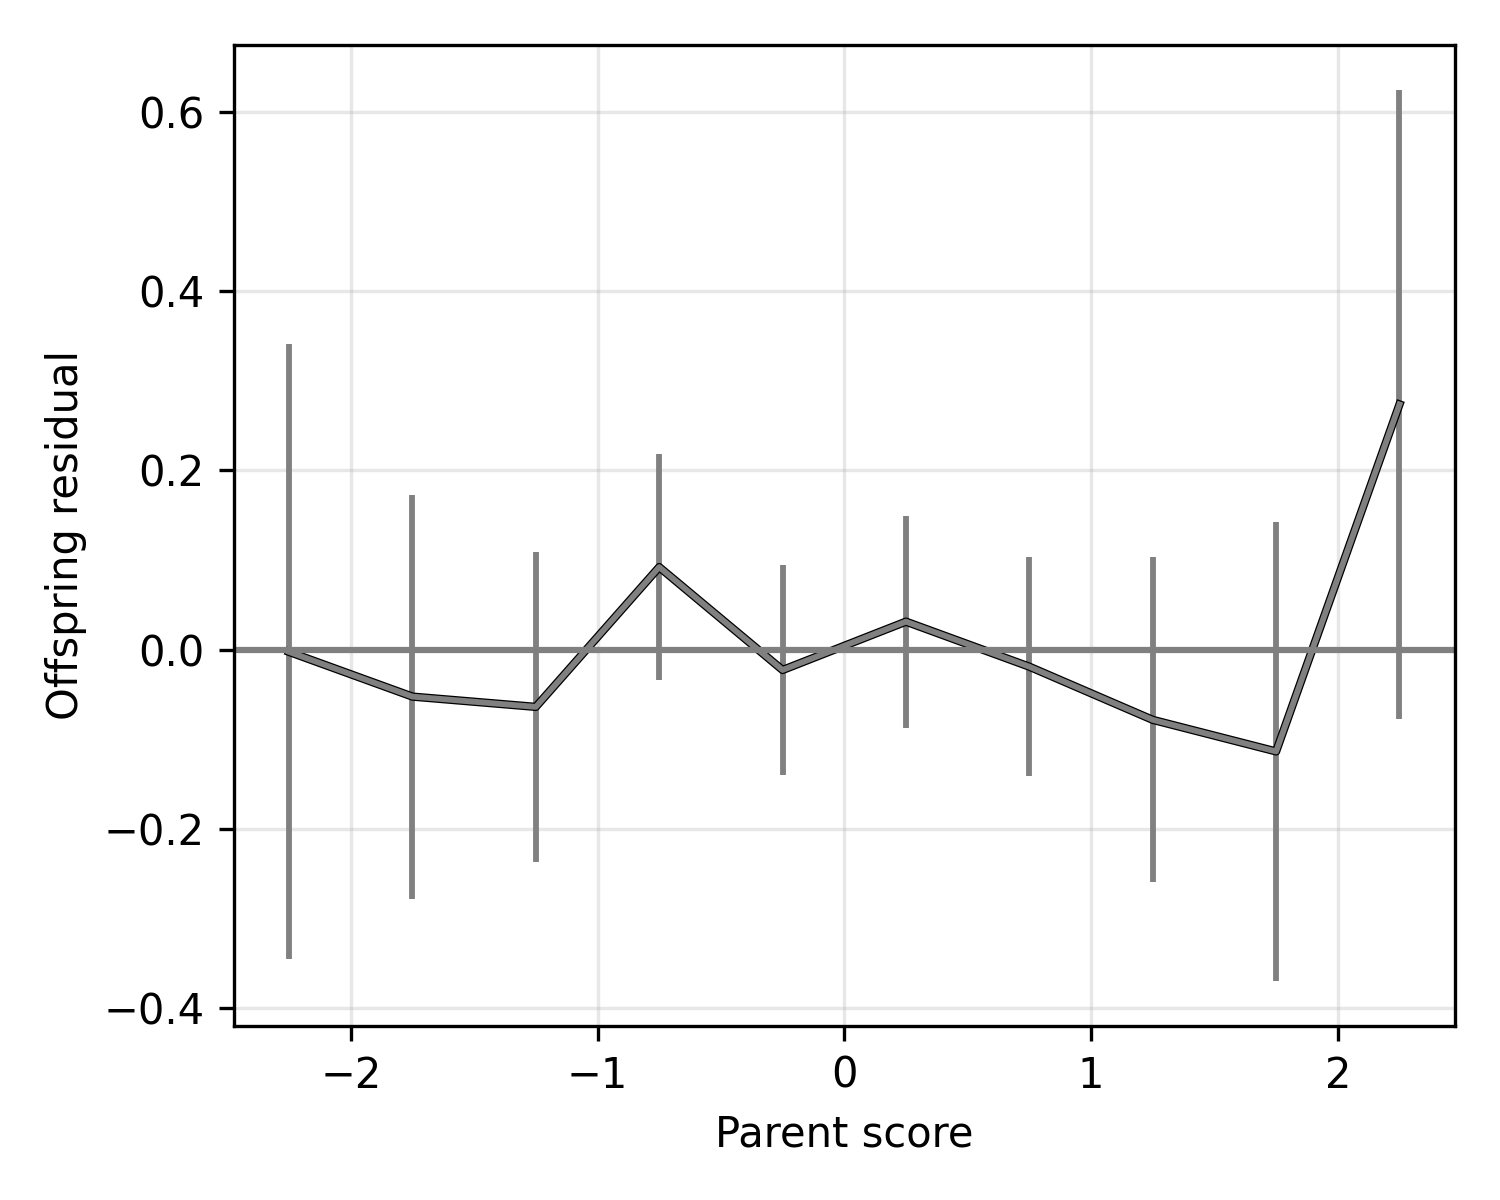
\includegraphics[width=3in]{figures/pearson_residuals_by_score.png}
\centering
\caption{Mean values of the residuals by parent score, shown with normal 95\% confidence intervals.}
\label{fig:pearson_residuals_by_score}
\end{figure}

The normality of the daughter generation was also confirmed by Q-Q plot, as well as skewness, kurtosis tests, and D’Agostino and Pearson's test.

In summary, we have confirmed from the Pearson female data both the initial condition and the one-step downward transition, and thus the entire model -- as long as there is stable population variance as described earlier. 


\subsubsection*{Observed coefficients and population variance dynamics}

The Pearson female data had the MLEs of $r$ = 0.54 and $r_s$ = 0.96, which nearly produce stable population variance (SD ratio of 1.10). Remarkably, $r^2 + r_s^2$ agreed with the variance of the daughters' scores to 15 decimal places -- the limit of the computer's output. However, the female data failed the F-test for equality of variances between the mother and daughter generation ($p < 0.01$). 

The Pearson male data had the MLEs of $r$ = 0.51 and $r_s$ = 0.89, which nearly produce stable population variance (SD ratio of 1.03). Again, $r^2 + r_s^2$ agreed with the variance of the sons' scores to 14 decimal places. The male data passed the F-test for equality of variances between the father and son generation ($p$ = 0.20). 

It is worth mentioning that the dataset collected by Francis Galton in 1885 was looked at, although it is not described in great detail here \cite{galton}. It contains the heights of 197 families and 898 adult children. For daughters-mothers ($n$ = 433), the SD ratio was 1.04 and had the MLEs of $r$ = 0.33 and $r_s$ = 0.99. This data passed the F-test for equality of variances between the mother and daughter generation ($p$ = 0.20). 

Overall, stable population variance seems \emph{a priori} to be a reasonable condition for human stature, though has mixed confirmation in actual data. One possible explanation for why the variance has sometimes been observed to be moderately larger in the offspring generation is that the offspring were relatively young adults, and so their heights may have continued to regress towards the mean after the study. Then, their eventual adult heights would have a more similar variance to the heights of their much older parents. This explanation is plausible because, in the Swedish data, all the adult children had their heights measured at around age eighteen. Similarly, in the Pearson data, the adult children had their heights measured when they were eighteen years of age or older. 

% Add citation to Karlberg
% https://www.nature.com/articles/pr1995278#citeas 









% MOBILITY AND INFORMATION LOSS
\section{Mobility and information loss}

We would like to find some way to quantify the degree of \emph{mobility} in the score of a descendant, given the score of its ancestor. This would also correspond to the \emph{loss of information} about the descendant's score, given its ancestor's score, or vice versa.

\subsection{Mobility as rate of convergence to the marginal distribution}
For the conditional descendant distribution, faster convergence means that the conditional distribution of the descendant's score quickly becomes indistinguishable from the marginal population distribution of its generation. Information that might precisely predict the descendant's score is \emph{lost} over the intervening generation(s). Faster convergence also means greater mobility, in that -- within few generations -- the descendant's distribution \emph{moves towards} the population distribution (both in expectation and variance). 

For the conditional ancestor distribution, faster convergence means that a descendant's score provides less information about its ancestor's score. 

\subsection{Proposed measure}
We have previously shown that convergence of the conditional distribution to the marginal distribution (both upward and downward) occurs faster with smaller $r$ and larger $r_s$ - and occurs slower for larger $r$ and smaller $r_s$. Accordingly, a simple measure of mobility and information loss would be proportional to $r$ and inversely proportional to $r_s$. 

Therefore, the simplest way to quantify the mobility and information loss that occurs between generations is with the following term:

\begin{description}
\item [Definition] Let $m$ be a measure of mobility or equivalently, a measure of information loss for the Markov chain with parameters $r$ and $r_s$:
$$m = \frac{r_s}{r}$$
\end{description}

In general, a value of $m$ is not unique to any given Markov chain, because infinitely many values for $r$ and $r_s$ can have the the same ratio. Although it is not investigated in detail here, different Markov chains with the same $m$ may turn out to have varied rates of convergence, upwards or downwards, or for expectation or variance. 

Nonetheless, for stable population variance (the stationary distribution), every possible Markov chain has a unique $m$. 
% Use case for M at the end. 

\subsection{Mobility under limiting cases}

We can show with some limiting cases for $r$ and $r_s$ that the desired effects in mobility and information loss occur, consistent with the proposed measure of mobility. 

\subsubsection*{Small regression coefficient}
Firstly, we consider the limiting case: $r \rightarrow 0$, causing $m \rightarrow \infty$. Then, for small $n$, we have:
$$X_{i+n}|X_i \rightarrow \mathcal{N}(0, \sigma_{i+n}^2)$$
In very few generations, there is nearly a complete loss in information about a descendant's score and there is maximum mobility. 

Likewise, there is also a nearly instantaneous complete loss of information about an ancestor's score, given its descendant's score:
$$X_{i-n}|X_i \rightarrow \mathcal{N}(0, \sigma_{i-n}^2)$$


\subsubsection*{Large residual coefficient}
Next, we consider the limiting case: $r_s \rightarrow \infty$, causing $m \rightarrow \infty$. Then, for small $n$, we have:
$$X_{i+n}|X_i \rightarrow \mathcal{N}(r^nX_i, \infty)$$
Note that the conditional variance rapidly the marginal variance, which goes to infinity:
$$ \tilde{\sigma}_{i+n}^2 \approx \sigma_{i+n}^2 \rightarrow \infty$$
Due to the extremely large variance of the marginal disribution, there is - almost instantly - a nearly complete loss in information about the descendant's score. There is also maximum mobility, as all conditional expectations would have z-scores of approximately zero. 

Likewise, there is also a complete loss in information about the ancestor's score, which converges to the marginal distribution:
$$X_{i-n}|X_i \rightarrow \mathcal{N}(0, \sigma_{i-n}^2)$$


\subsubsection*{Small residual coefficient}
Lastly, we consider the limiting case: $r_s \rightarrow 0$. Because of the degenerate lower bound on $r_s$, shown in Figure \ref{fig:possible_r_rs}, there are two ways for the residual coefficient to approach zero, either the regression coefficient approaches its lower bound of zero, or its upper bound of one.

In the first case: $r \rightarrow 0$, it is straightforward to show form the degenerate bound that $r$ must shrink to zero faster than $r_s$ shrinks to zero, such that, if $r$ is made as close as possible to the degenerate bound ($r$ is as great as it possibly can be), we get:
$$r_s^2 \approx r$$
Then, our measure of mobility and information loss still goes to infinity:
$$m \approx \frac{1}{r_s} \rightarrow \infty$$
Indeed, there is rapid downward convergence to the marginal distribution. For small $n$, we have:
$$X_{i+n}|X_i \rightarrow \mathcal{N}(0, \sigma_{i+n}^2)$$
Likewise, there is also a complete loss in information about the ancestor's score, due to the extremely large population variance and an upper limit on the conditional expectation, such that $\tilde{\mu}_{i-n} < X_i$:
$$X_{i-n}|X_i \rightarrow \mathcal{N}((\frac{r}{r^2+r_s^2})^n X_i, \infty)$$
$$\tilde{\sigma}_{i-n}^2 \approx \sigma_{i-n}^2 \rightarrow \infty$$


In the second case: $r \rightarrow 1$, we get the smallest amount of mobility and information loss. That is, $m \rightarrow 0$. For small $n$, we have:
$$X_{i+n}|X_i \rightarrow \mathcal{N}(X_i, 0)$$
$$X_{i-n}|X_i \rightarrow \mathcal{N}(X_i, 0)$$
Because we also have $r^2 + r_s^2 \rightarrow 1$, the second case is consistent with stable population variance and the stationary distribution.
$\sigma_{i-n}^2 \approx \sigma_{i-n}^2 \approx 1$
In other words, there is nearly no mobility whatsoever between generations, and very little information is lost about a descendant's or an ancestor's score between generations. That is, an ancestor's score gives an almost perfect prediction of its descendant's score, and vice versa.




%% PROBABILITY KERNELS %%
\section{Probability kernels}

\subsection{State to set probability}
Let $A$ be a subset of the state space: 
%
$$A \subseteq \mathbb{R}$$

\begin{description}
\item [Definition] The probability kernel $P_n(A, x_i)$ is the $n$-step probability of reaching the set $A$ from the state $x_i$.
$$P_n(A, x_i) = \int_{x_{i+n}\in A}^{} f(x_{i+n}|x_i)f(x_i) \, dx_{i+n}$$
\end{description}

Where $f(x_{i+n}|x_i)$ is the conditional probability density function (pdf) of $X_{i+n}|X_i \sim \mathcal{N}( \tilde{\mu}_{i+n}, \tilde{\sigma}_{i+n})$, and $f(x_i)$ is the pdf of $X_i \sim \mathcal{N}(0, \sigma_i^2)$.
The expression can be simplified to the following, as long as $A$ is the uninterrupted set $(A_{min}, A_{max})$:

$$P_n(A, x_i) = f(x_i)[\, \Phi(\frac{A_{max}- \tilde{\mu}_{i+n}}{\tilde{\sigma}_{i+n}}) - \Phi(\frac{A_{min}- \tilde{\mu}_{i+n}}{\tilde{\sigma}_{i+n}}) \, ]$$

Where $\Phi$ is the cumulative density function (cdf) of the standard normal distribution. 


\subsection{Set to set probability}
Let $B$ also be a subset of the state space:
%
$$B \subseteq \mathbb{R}$$

\begin{description}
\item [Definition] A similar probability kernel $P_n(A, B)$ is the $n$-step probability of reaching the set $A$ from the set $B$. 
$$P_n(A, B) = \int_{x_i\in B}^{} P_n(A, x_i) \, dx_i$$
\end{description}




% ATTRIBUTABLE
\subsection{Probability attributable}

\begin{description}
\item [Definition] $P_{\alpha , n}(A, B)$ is the probability that a state $X_{i+n}$ in set $A$ came from or is \emph{attributable} to an ancestor state $X_i$ in set $B$.
$$P_{\alpha , n}(A, B) = \frac{P_n(A, B)}{P_n(A, \mathbb{R})}$$
\end{description}

By the law of total probability, $P_n(A, \mathbb{R})$ is the marginal probability that the state $X_{i+n}$ is in the space $A$, this can be obtained by the cumulative density function of a normal distribution by the following definition.

\begin{description}
\item [Definition] For some arbitrary subset of the state space $S \subseteq \mathbb{R}$, $P(S)$ is the marginal probability that the normally distributed rv $X \sim \mathcal{N}(\mu, \sigma^2)$ is in the subset $S$. The last equality holds if $S$ is the uninterrupted set $(S_{min}, S_{max})$.
$$P(S) = \int_{x\in S} f(x) \, dx = \Phi(\frac{S_{max} - \mu}{\sigma}) - \Phi(\frac{S_{min} - \mu}{\sigma})$$
\end{description}

For $P(A)$, its integrand $f(x)$ would be the pdf of $X_{i+n} \sim \mathcal{N}(0, \sigma_{i+n}^2)$. Therefore:
%
$$P_{\alpha , n}(A, B) = \frac{P_n(A, B)}{P(A)}$$

% DESTINED
\subsection{Probability destined}

\begin{description}
\item [Definition] $P_{\delta , n}(A, B)$ is the probability that a state $X_i$ in set $B$ has a descendant state $X_{i+n}$ that appears in or is \emph{destined} for the set $A$. 
$$P_{\delta , n}(A, B) = \frac{P_n(A, B)}{P_n(\mathbb{R}, B)}$$
\end{description}

It can be shown by the fact that an integral over the entire support of a pdf equals one, that $P_n(\mathbb{R}, B)$ is the marginal probability that the state $X_i$ is in the set $B$, which is given by $P(B)$. Therefore:
%
$$P_{\delta , n}(A, B) = \frac{P_n(A, B)}{P(B)}$$


\subsubsection*{Note about unstable population variance}
Probability attributable and destined calculations are generally made on a relative basis, which means they are not affected by unstable population variance. Specifically, the sets $A$ and $B$, and are usually stated in terms of percentiles, as we shall see. In that case, the descendant population, for which the set $A$ is a part of, may have an absurdly large or small variance relative to the set $B$ is a part of, but the ratio in variances is made irrelevant due to standardization.


\subsection{Percentile transiton matrices}

The calculations of probability attributable and probability destined can be defined by percentiles with sets $A$ and $B$ generally calculated relative to the populations they are a part of. For example, in $P_{\delta , n}(A, B)$, the state $B$ would be calculated as a percentile, relative to the marginal population variance $\sigma_i^2$ of generation $i$. 

Such percentile-based calculations can be used to create percentile transition matrices. As the states would be calculated from percentiles and all percentiles in the matrix would be the same, e.g. 20\%, then $P(A) = P(B)$ for all calculations. Therefore, in percentile transition matrices, probability attributable calculations are identical to probability destined calculations.
$$P_{\alpha , n}(A, B) = P_{\delta , n}(A, B)$$

In Figure \ref{fig:old_quintile_p1}, we see an example of a quintile transition matrix showing the probability that an offspring's score is within a certain quintile, e.g., the bottom quintile, the middle quintile, etc., given the quintile of its parent's score. As described just a moment ago, the Figure \ref{fig:old_quintile_p1} is equally a plot of probability destined. That is, it is also showing probability that a parent's score is within a certain quintile, given the quintile of its offspring's score (mentally switch the words \emph{offspring} and \emph{parent} when looking at the Figure \ref{fig:old_quintile_p1}).

\begin{figure}[h]
\centering
\advance\leftskip+0.8cm
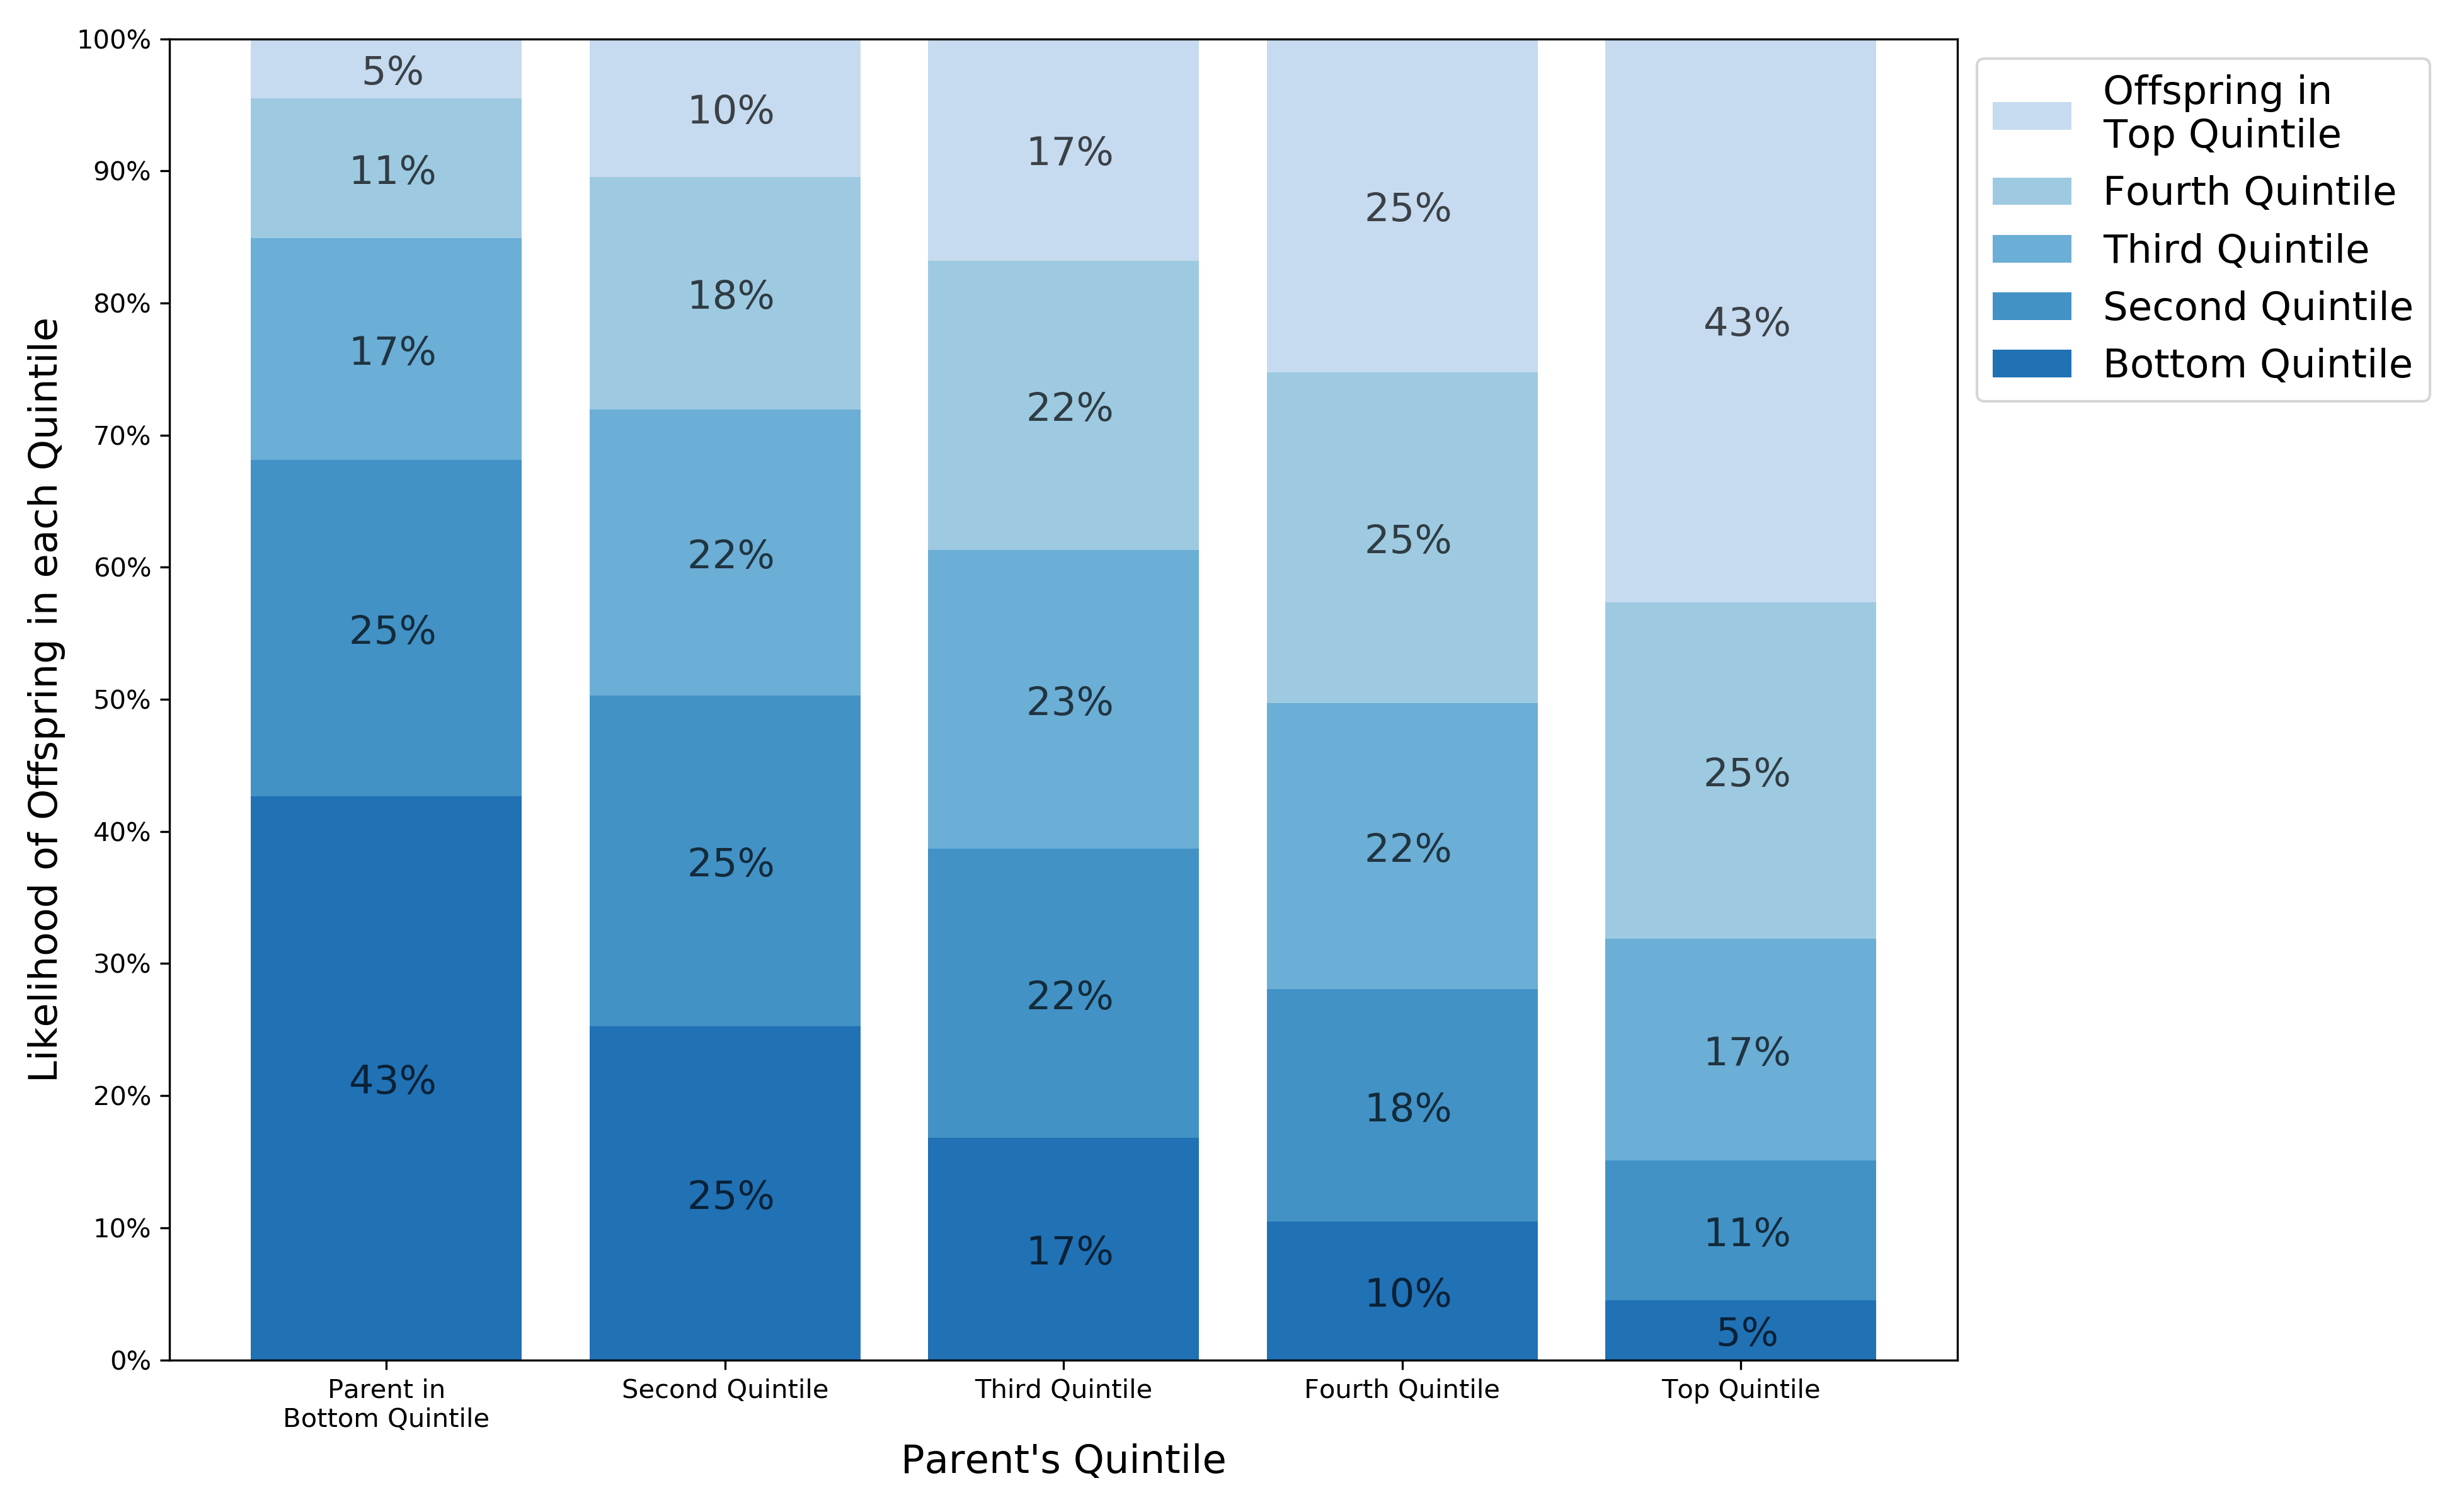
\includegraphics[width=0.8\linewidth]{figures/model_mobility_n1000_r50_r_s90_.png} 
\caption{Example of a probability attributable quintile transition matrix, with parameters $r = 0.5$ and $r_s = 0.9$.}
\label{fig:old_quintile_p1}
\end{figure}

The parameters quintile transition matrix in \ref{fig:old_quintile_p1} can be compared with the calculated values of the the dataset collected by Francis Galton in 1885, shown in  \ref{fig:old_galton_quintile} (197 families and 898 adult children). 

\begin{figure}[h]
\centering
\advance\leftskip+0.8cm
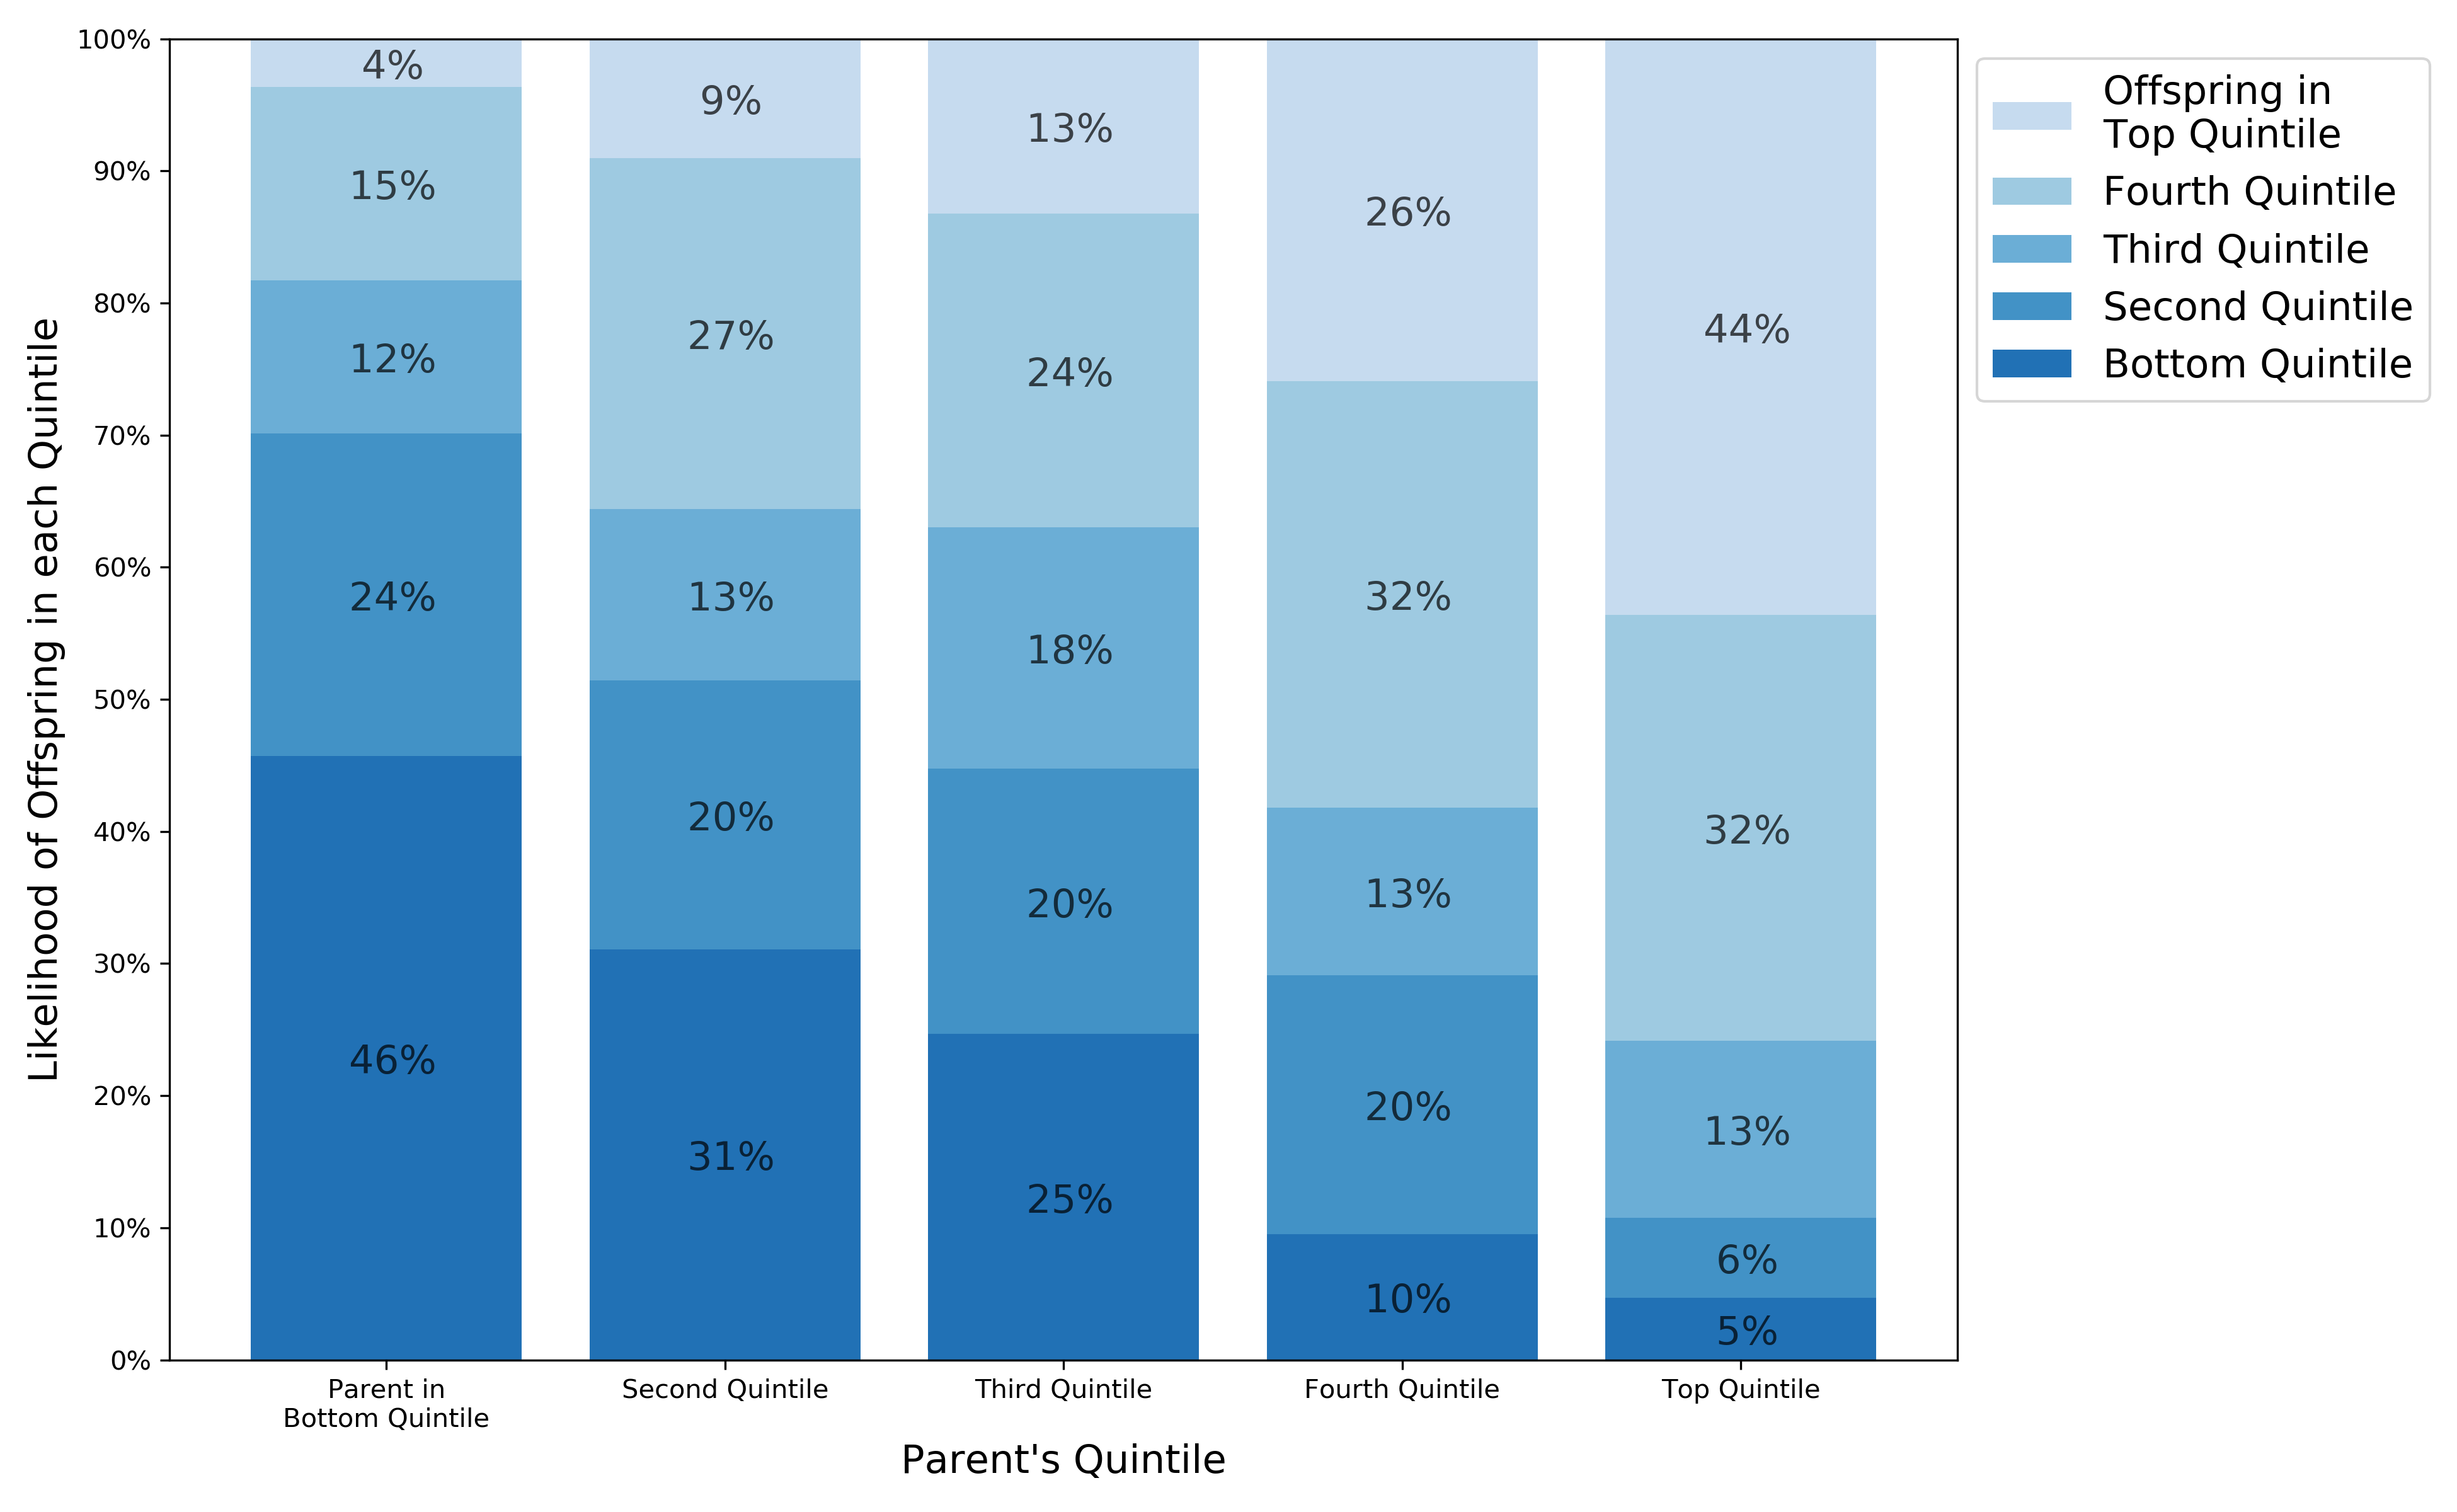
\includegraphics[width=0.8\linewidth]{figures/galton_mobility.png} 
\caption{Calculated transition matrix from data on the heights of 898 adult children and their 394 parents. Observed parameters $r = 0.51$ and $r_s = 0.90$ (using midparental heights for the regression).}
\label{fig:old_galton_quintile}
\end{figure}


The effect of $m$ in determining mobility and information loss becomes clear as the regression and residual coefficients determine the percentile transition matrices. While an example is not given here, percentile transition matrices can be calculated for any number of generations $n$ separating the ancestor and descendant. 

Multi-generational transition matrices are forthcoming.

\section{Discussion}
Forthcoming.





\clearpage


% APPENDIX
\section{Appendix}

\subsection*{Check with Eve's law}
We can verify our expression for $\mathrm{Var}(X_{i+n})$ using Eve's law:
%
$$\mathrm{Var}(X_{i+n}) = \mathrm{E}(\mathrm{Var}(X_i|X_{i+n})) + \mathrm{Var}(\mathrm{E}(X_{i+n}|X_i))$$
%
As we have previously shown:
%
$$\mathrm{E}(\mathrm{Var}(X_{i+n}|X_i)) = \sigma_i^2 [(r^2+r_s^2)^n-r^{2n}]$$
$$\mathrm{Var}(\mathrm{E}(X_{i+n}|X_i)) = \mathrm{Var}(r^nX_i) = r^{2n}\sigma_i^2$$
%
Combining the terms, we confirm our earlier expression:
%
$$\sigma_{i+n}^2 = (r^2+r_s^2)^n  \sigma_i^2$$


\subsection*{Use cases}
With the two coefficients $r$ and $r_s$, we can perfectly describe the variance of the offspring's generation relative to that of the parent's generation through the following relation:
%
$$\frac{\sigma_{i+1}^2}{\sigma_i^2} = r^2+r_s^2$$
%
Simply knowing or having measured two of the three values: the ratio parent generation and offspring generation variance, the regression coefficient ($r$), the residual coefficient ($r_s$); it is possible to obtain the third.
%
This can be useful, for example, to obtain the SD of the offspring's polygenic score, after having measured the parent's polygenic score: $\tilde{\sigma}_{i+1} = r_s \sigma_i$.
%
Alternatively, after having only measured the $\frac{\sigma_{i+1}^2}{\sigma_i^2}$, which is one when there is stable population variance, and $r$, which can be obtained through ordinary least squares with the parent and offspring data or by the correlation coefficient between parent and offspring when there is stable population variance; the model can be constructed and applied.


\subsubsection*{Stationary distribution use case}
Under stable population variance, observing or measuring one of $r$ or $r_s$ immediately gives away the other. As an example, $r$ could be obtained by the correlation coefficient between parent and offspring.  
$$\mathrm{Corr}(X_{i+1}, X_i) = r$$

Alternatively, $r$ could be obtained by ordinary least squares, as described later.

When there is stable population variance, knowledge of either $r$ or $r_s$ provides sufficient information to model the population with the proposed Markov chain model.





\clearpage


%\begin{verbatim}
%Put your R code here.
%\end{verbatim}

\bibliographystyle{apalike}
\bibliography{polygenic_bib}


\end{document}

% Notes to self:
% Distributed iid: \stackrel{iid}{\sim}
